%% LyX 2.2.1 created this file.  For more info, see http://www.lyx.org/.
%% Do not edit unless you really know what you are doing.
\documentclass[11pt,english]{article}
\usepackage[T1]{fontenc}
\usepackage[latin9]{inputenc}
\usepackage{amsmath}
\usepackage{amsthm}
\usepackage{amssymb}
\usepackage{graphicx}
\usepackage{setspace}
\usepackage{esint}
\usepackage[authoryear]{natbib}
\onehalfspacing

\makeatletter

%%%%%%%%%%%%%%%%%%%%%%%%%%%%%% LyX specific LaTeX commands.
%% Because html converters don't know tabularnewline
\providecommand{\tabularnewline}{\\}

%%%%%%%%%%%%%%%%%%%%%%%%%%%%%% User specified LaTeX commands.
\usepackage{amsthm}\usepackage{times}
\usepackage{graphicx}
\usepackage{amsfonts}\usepackage{babel}\usepackage{wasysym}

\textwidth6.5in\textheight9in\oddsidemargin-0.0in\topmargin-0.5in\linespread{1.5}


%Different font in captions
\newcommand{\captionfonts}{\small}

\makeatother

\usepackage{babel}
\renewcommand\theenumi{(\alph{enumi})}
\renewcommand\labelenumi{\theenumi}

%\usepackage{tikz}
%\usetikzlibrary{arrows, positioning}

% Nils preamble
%\documentstyle{article}%\pagestyle{empty}                    % No page numbering

\usepackage{comment}
\usepackage{graphicx}


\usepackage{float}
\usepackage{lscape}
%\usepackage{arydshln}


\usepackage{bbm}%For indicator function


\usepackage{amsthm}
\usepackage{bm}


\usepackage{array}
\usepackage{multirow}
%\usepackage{latexsym}
\oddsidemargin 0.0in                % Extra space added to the left for binding
\topmargin -.75in
\renewcommand{\baselinestretch}{1.43}%{1.43}
\setlength{\textwidth}{6.75in}
\setlength{\textheight}{9.25in}
\parskip0pt                          % Extra vertical space between paragraphs.
\parindent0pt                       % Width of paragraph indentation.
%\topsep -10pt plus .5pt minus .5pt     % Extra vertical space, in addition to
                                     % \parskip, added above and below list and
                                     % paragraphing environments.
%\partopsep -90pt %plus .5pt minus .5pt  % Extra vertical space, in addition to
                                     % \parskip and \topsep, added when user
                                     % leaves blank line before environment.
%\itemsep=-50pt
%\itemsep -90pt plus -10pt                % Extra vertical space, in addition to
                                     % \parskip, added between list items.
\newtheorem{theorem}{T{\scriptsize HEOREM}}\newtheorem{corollary}{C{\scriptsize OROLLARY}}\newtheorem{proposition}{P{\scriptsize ROPOSITION}}\newtheorem{lemma}{L{\scriptsize EMMA}}\newtheorem{definition}{D{\scriptsize EFINITION}}\newtheorem{claim}{C{\scriptsize LAIM}}

\makeatother

\usepackage{babel}
\begin{document}

\title{Measuring the Impact of Shot Sequencing on First Mover Advantage
in Penalty Shootouts \thanks{Thanks here}}

\author{Nils Rudi\\
\textit{\small{}Insead}\and Aditya Shetty\\
\textit{\small{}University of Rochester}\and Marcelo Olivares\\
\textit{\small{}Universidad de Chile} \textit{\small{}}}

\maketitle
\vspace{-8mm}

\begin{abstract}
Lorem ipsum. 

\textbf{Keywords}: sport science, applied econometrics, psychological
pressure
\end{abstract}
\thispagestyle{empty}

\newpage{}% blank page for back side of title page

\setcounter{page}{1} \global\long\global\long\global\long\global\long\global\long\global\long\global\long\global\long\def\baselinestretch{1.5}


\section{Introduction }

\label{sec:intro}

REWRITE THIS PART

About 26.5\% of football games are tied at the end of the normative
90 minutes. When a winner is required\textemdash typically in elimination
tournament format \textendash{} such games will go on to normative
30 additional minutes. If a winner is still not determined, the match
will go to a penalty shootout. Here the teams will take alternating
penalties, i.e., first team A then team B and so it goes. This sequence
is coined ABAB. Team A used to be determined by the outcome of a coin
flip, while since 2003 a coin flip determines which team's captain
will get to choose the sequence.

Penalty shootouts is however a process that receives some controversy.
Criticism include that it only reflects a narrow part of the game\textemdash and
hence that the criteria does not reflect the rich game, and that it
seems to be to a large extent a game of chance\textemdash i.e., that
it does not really differentiate much even within the narrow slice
of the game. On the positive aspects is the spectacular drama\textemdash with
shooter vs. goalie in person-to-person duels, it is an easy to understand
format, and a winner is indeed determined in a reasonable amount of
time.

This paper focus on another criticism\textemdash namely that team
A tends to get an advantage, claimed by some to be an {\em unfair}
aspect of the penalty shootout. This advantage is demonstrated to
be 60.5\% in 269 matches by AER. Using an extended dataset of 540
matches, MS finds that team A wins in 53.3\% of the cases, while with
an even larger dataset of 1,001 matches, BOOK finds the team A advantage
to be 60.6\%.

Wether or not such an advantage is unfair is a question of definition.
LITERATURE ON FAIRNESS. The outcome of a football match is determined
by factors that roughly can separated into two groups. One is factors
internal to the game, such as a kick on the ball, a defender covering
space and a shot hitting the goal post. The other is factors external
to the game, or {\em deus ex machina}, such as one team playing
against the sun in first half and the second half being played after
sunset. In general it is desirable that the outcome of a match is
determined by internal factors, and that the impact of external factors
is minimized. While a coin flip is probabilistically fair\textemdash it
is even called a {\em fair coin}\textemdash it is a factor external
to the game. Alternative sequences may reduce the impact of the coin
flip but potentially at the cost of complexity of less structure in
the sequence as ABAB arguable is one of the simplest possible.

IFAB is the governing body of the football rules. To make a major
change in the rules requires at least six of the total eight votes,
which consist of FIFA's four votes and one vote for each of the four
British football associations. IFAB is currently considering alternative
sequences for the penalty shootout, and there has been recent experiments
with ABBA in XYZ tournaments.

The main objective of this paper is to investigate the impact of alternative
sequences of penalty shootouts. A a dataset of X shootouts of shot-by-shot
outcomes enables us to do a detailed analysis of the impact of sequence
and model alternative sequences.

TO INCLUDE IN THE INTRO:

Example of penalty shootouts in soccer. Evidence in previous work.

This paper:
\begin{itemize}
\item Reevaluate first mover advantage in shootouts, expanding the dataset
of APH and Kocher Lenz Sutter.
\item Analyze shot-by-shot to: (1) understand the underlying mechanisms
driving the first mover advantage. (2) use the estimates to evaluate
alternative sequences of shots in order to reduce first-mover advantage.
\end{itemize}

\section{Data and Shootout level analysis\label{sec:data}}

This section describes the data collection scheme and provides the
empirical estimates of the first-mover advantage, comparing to the
results of previous work.

\subsection{Data collection\label{subsec:datacoll}}

\citet{kocher2012psychological} showed that the data collection process
can influence the magnitude and statistical significance of the effect
of first-mover advantage. For this reason, the analysis in this work
was divided into two data collection schemes. The first dataset is
comprised of the same competitions used in \citet{apesteguia2010psychological}
and \citet{kocher2012psychological}. These data collection starts
with the dataset used in \citet{kocher2012psychological} (a superset
of \citet{apesteguia2010psychological}) and expands using multiple
data sources.\footnote{We thank the authors of \citet{kocher2012psychological} for providing
their dataset.} We refer to this dataset as the APH competitions data. A second data
collection scheme incorporates additional adult male competitions
for which we could obtain a reasonable number of shootouts (10 shootouts
our more during 1970-2017. This dataset is refered as the extended
competitions data., and the additional competitions are listed in
the Appendix Table \ref{tab:add_comp}. 

The data was collected at two levels of granularity. At a more aggregate
level, shootout-level data can be used to test whether the starting
team wins more frequently. For this purpose, the sample of shootouts
requires (at least) information about the tournament of the match,
the team that took the first shot and the outcome of the shootout
(which team won). Specific details about the name of the team, the
date of the match, the championship round and the final score are
not required to conduct the test but can be useful to include as control
variables. This level of aggregation has been used to test for a first-mover
advantage ( \citet{kocher2012psychological}, \citet{apesteguia2010psychological}\footnote{}). 

More detailed data include the outcome of every shot taken in the
shootout. This information can be useful to understand further details
of the mechanisms driving the first mover advantage, analyzing how
the shooting performance of player is affected by the order of shooting,
goal difference between the teams, shooting round, among other factors.
This detailed information is available for a subset of the shootouts
included in the final sample. \citet{apesteguia2010psychological}
also used shot-by-shot information to compare the shooting performance
of the starting and second team across rounds. We significantly expanded
the number of shootouts to conducts this analysis and also construct
new measures that help to explain the underlying mechanism driving
the first-mover advantage.

<\textcompwordmark{}<DESCRIPTION ON HOW THE ONLINE DATA WAS COLLECTED
GOES HERE. INDICATE WHAT WAS DONE FOR THE AER COMPETITIONS AS WELL
AS THE EXTENDED SET OF COMPETITIONS WE CONSIDER {*}{*} ADITYA, PLEASE
COMPLETE {*}{*}>\textcompwordmark{}>

The data available through online sources under-represents the shootouts
for the Spanish League. This is relevant because \citet{kocher2012psychological}
shows this tournament has the highest proportion of starting team
winners. To collect more data on that tournament, four sources of
newspapers were revised. In total, XXX additional matches were collected,
for which YYY also had information on the order of the shots. <\textcompwordmark{}<
ADITYA, PLEASE COMPLETE THIS INFO WITH THE ANALYSIS YOU DID>\textcompwordmark{}>

Table \ref{tab:summstats} reports a summary of the shootouts for
each of the APH competitions, describing the number of shootouts found
where the starting team information was available. The table also
reports fraction of matches won by the starting team and the p-value
of a one-sided binomial test of the null $H_{0}:p=0.5$ against the
one-sided alternative $H_{1}:p>0.5$. The one-sided test is more appropriate
in this case, since the test is to identify an advantage of the starting
team.

Overall, the data suggests an advantage for the starting team of about
10\% (55\% vs 45\%), that is, 22\% more likely to win. The proportion
of wins of the starting team is highly statistically significant above
50\% at the 0.1\% level for the overall sample. This proportion is
similar for international and league teams.

The total is sample size is 970, compared to the 540 matches studied
in \citet{kocher2012psychological}. In most of their analysis, \citet{apesteguia2010psychological}
and \citet{kocher2012psychological} restrict their sample up to 2003
in order to have a clean natural experiment. Before 2003, the winner
of the toin-coss had to start the shootout, but after 2003 the winner
could \emph{choose} to go first or second. \citet{apesteguia2010psychological}
reports that in most cases the winner of the toss chooses to go first.
Although the post-2003 is not a perfect natural experiment, it seems
reasonable to use this period to increase the statistical power of
the tests, which is considered in part of the analysis reported in
\citet{apesteguia2010psychological}, as we do.

<\textcompwordmark{}<{*}{*}ADITYA, NILS: please include here your
analysis on the sample selection.

{*}{*}NOTE MO: Our sample covers until 2016? 2017?. Kocher studies
until 2003, they cover 540 matches out of a universe of 709. What
is the universe of matches in our case? That is: how many matches
with shootouts did we not obtain outcome data because info was not
available? How many additional could we get prior to 2003? We should
separate the table pre and post 2003. After we do that, we should
do a comparison of the pre-2003 sample with Kocher.>\textcompwordmark{}>.

\citet{palacios2014beautiful} reevaluates the first-mover advantage
using the same tournaments as \citet{apesteguia2010psychological},
expanding the dataset from 156 shootouts to 1001, covering matches
up to 2012. <\textcompwordmark{}< {*}{*}{*} NOTE MO: Do a comparison
of the samples. On national teams, seems like we have similar composition
{*}{*}{*}.>\textcompwordmark{}>. The data in \citet{palacios2014beautiful}
shows that 60.6\% percent of the matches were won by the starting
team, similar to the previous result obtained by \citet{apesteguia2010psychological}
which uses only pre-2003 matches. The first-mover advantage in \citet{palacios2014beautiful}
seems to be substantially higher that the one obtained with our sample
(55.7\%), which is in between their estimate and the 53.3\% reported
in \citet{kocher2012psychological}.

\begin{table}
\begin{tabular}{cccccc}
\textbf{competition} &  & \textbf{n} & \textbf{Mean} &  & \textbf{p-value}\tabularnewline
\emph{League teams} &  &  &  &  & \tabularnewline
Champions League &  & 33 & 60.61\% &  & 0.0814\tabularnewline
Champions League Qual. &  & 18 & 66.67\% &  & 0.0481\tabularnewline
Copa del Rey &  & 256 & 60.94\% &  & 0.0002\tabularnewline
Cup Winners Cup &  & 29 & 58.62\% &  & 0.1325\tabularnewline
DFB-Pokal &  & 206 & 50.00\% &  & 0.4722\tabularnewline
Europa League &  & 90 & 52.22\% &  & 0.2992\tabularnewline
Europa League Qual. &  & 42 & 52.38\% &  & 0.3220\tabularnewline
FA Community Shield &  & 6 & 50.00\% &  & 0.3438\tabularnewline
FA Cup &  & 37 & 43.24\% &  & 0.7443\tabularnewline
League Cup &  & 142 & 58.45\% &  & 0.0178\tabularnewline
 &  &  &  &  & \tabularnewline
\emph{National teams} &  &  &  &  & \tabularnewline
Africa Cup &  & 23 & 52.17\% &  & 0.3388\tabularnewline
Asian Cup &  & 12 & 50.00\% &  & 0.3872\tabularnewline
Copa Am�rica &  & 20 & 65.00\% &  & 0.0577\tabularnewline
EURO &  & 18 & 44.44\% &  & 0.5927\tabularnewline
Gold Cup &  & 12 & 66.67\% &  & 0.0730\tabularnewline
World Cup &  & 26 & 57.69\% &  & 0.1635\tabularnewline
 &  &  &  &  & \tabularnewline
League Teams &  & 859 & 55.76\% &  & 0.0003\tabularnewline
National teams &  & 111 & 55.86\% &  & 0.0918\tabularnewline
 &  &  &  &  & \tabularnewline
Total &  & 970 & 55.77\% &  & 0.0001\tabularnewline
 &  &  &  &  & \tabularnewline
\end{tabular}

\caption{Summary statistics of shootouts for APH competitions, showing the
percent of matches where the starting team wins the shootout.\label{tab:summstats}}
\end{table}

In addition to the simple t-tests reported in Table \ref{tab:summstats},
a linear probability was used to test for the first-mover advantage
including dummy variables of year and competition as control variables.
The results are summarized in Table \ref{tab:results_LPM}, corroborating
the findings of the summary statistics and suggesting a 10\% advantage
for the starting team (55\% vs. 45\%). If we restrict the sample to
matches before 2003 (reported in the second column), the effect of
starting team is also statistically significant and similar in magnitude.

\begin{table}
\centering{
\def\sym#1{\ifmmode^{#1}\else\(^{#1}\)\fi}
\begin{tabular}{l*{2}{c}}
\hline\hline
                    &\multicolumn{1}{c}{(1)}&\multicolumn{1}{c}{(2)}\\
                    &\multicolumn{1}{c}{WinH}&\multicolumn{1}{c}{WinHpre2003}\\
\hline
FirstShot           &       0.117\sym{***}&       0.165\sym{**} \\
                    &    (0.0330)         &    (0.0499)         \\
\hline
Observations        &         970         &         438         \\
\hline\hline
\multicolumn{3}{l}{\footnotesize Robust standard errors. Includes dummies for competition and year}\\
\multicolumn{3}{l}{\footnotesize \sym{*} \(p<0.05\), \sym{**} \(p<0.01\), \sym{***} \(p<0.001\)}\\
\end{tabular}
}


\caption{Estimation results for Linear Probability Model, APH competitions
\label{tab:results_LPM} }
\end{table}

The estimation was replicated using the extended competition dataset,
increasing the number of shootouts to 1698. The results are similar,
suggesting a 12.5\% advantage of the starting team. When restricting
the sample to matches before 2003, the effect appears to be larger,
above 20\%. <\textcompwordmark{}< {*}{*} ADITYA, NILS: in the pre2003
shootouts, the sample increased only from 438 to 534, whereas for
the whole period it increased from 970 to 1698. Clearly the new data
is mostly for post 2003. It would be useful to have a more detailed
description of the competitions that were added pre2003 and perhaps
explain why the first mover advantage is so large for these {*}{*}
>\textcompwordmark{}>

Overall, the additional data considered in this study suggests a winning
advantage of the first-shooting team of 55\% vs. 45\% for the second
team. This estimate is statistically significant but smaller than
the results reported in \citet{apesteguia2010psychological} and \citet{palacios2014beautiful};
our result is closer to the estimate of \citet{kocher2012psychological}.

\section{Shot-by-shot empirical analysis\label{sec:shotbyshot}}

The previous section uses a shootout as the main unit of analysis.
The analyses revealed a significant and robust effect of first-mover
advantage in the shootouts, which settles part of the controversy
reported in previous studies. An additional objective of this work
is to conduct a counterfactual analysis to study how a change in the
sequence would affect this first mover advantage; this requires a
more detailed understanding of the underlying mechanisms driving this
advantage. To do so, we use outcomes of individual shots in penalty
shootouts to analyze how the performance of shooters is affected by
different conditions in which the shots are taken, including the round
and partial result of the shootout.

\subsection{First-mover advantage by shooting round}

For a subset of the shootouts, the outcome of each shot, $y_{ijt}$,
is recorded for match $i$ by team $j$ in round $t$, where a value
equal to one indicates that the shot is scored. Teams are indexed
by $j=\{1,2\}$ , where $j=1$ is the starting team in the shootout.
The rounds $t=\{1\ldots5\}$ may determine the winner if the accumulated
number of goals $Y_{ij5}=\sum_{t=1}^{5}y_{ijt}$ is strictly greater
for one of the two teams; otherwise rounds $t\geq6$ are completed
until one of the teams gets a goal advantage at the end of the round.

First, we verify the prevalence of the first mover advantage in this
shot-level analysis. A binary variable is included in the model indicating
if the team started first, $ShotFirst$, which is equal to one for
team $j=1$. The overall scoring performance is 73.4\%. Table \eqref{tab:results_shotbase}
show summary statistics of the fraction of scored shots for the first
and second shooter, on each of the first 5 rounds and beyond that
(6+). The dataset include 905 shootouts with sequence. Some of these
shootouts end before the 5th round; for example, with a score of 3-0
after the second shot in the third round the shootout ends. Therefore,
the number of shots decreases for later rounds, and some of them stop
with the first shot (so that the second team did not take the shot). 

The table reveals that on each round, the shooting performance is
higher for the first shot. The difference between first and second
shot becomes larger after the second round, which is mostly explained
by a reduction in the performance of the second team, dropping from
75\% to 70\% (approximately). The t-statistic for test of equal proportions
is included along with the corresponding p-value of the one-sided
t-test. The difference in shooting performance is statistically significant
at the 5\% level for the third and fifth round and for the overall
sample. These results are in line with those found in \citet{apesteguia2010psychological},
who also find a higher difference in shooting performance for the
later rounds in the shootout.

\begin{table}
\caption{Summary statistics of shot performance for first and second shooter,
by round. APH competitions data.\label{tab:summstat_shot}}

\centering%
\begin{tabular}{cccccc}
\hline 
Round & first & second & Difference & t-stat & p-value\tabularnewline
\hline 
 &  &  &  &  & \tabularnewline
1 & 75.7\% & 74.9\% & 0.9\% & 0.43 & 0.335\tabularnewline
 & 907 & 907 &  &  & \tabularnewline
 &  &  &  &  & \tabularnewline
2 & 75.1\% & 74.3\% & 0.8\% & 0.37 & 0.355\tabularnewline
 & 907 & 907 &  &  & \tabularnewline
 &  &  &  &  & \tabularnewline
3 & 74.8\% & 70.1\% & 4.6\% & 2.23 & 0.013\tabularnewline
 & 907 & 907 &  &  & \tabularnewline
 &  &  &  &  & \tabularnewline
4 & 74.3\% & 70.9\% & 3.4\% & 1.59 & 0.056\tabularnewline
 & 894 & 817 &  &  & \tabularnewline
 &  &  &  &  & \tabularnewline
5 & 75.0\% & 69.3\% & 5.7\% & 2.19 & 0.014\tabularnewline
 & 692 & 485 &  &  & \tabularnewline
 &  &  &  &  & \tabularnewline
6+ & 73.4\% & 70.5\% & 2.9\% & 1.10 & 0.136\tabularnewline
 & 545 & 545 &  &  & \tabularnewline
 &  &  &  &  & \tabularnewline
Total & 74.8\% & 72.0\% & 2.8\% & 3.09 & 0.001\tabularnewline
 & 4852 & 4568 &  &  & \tabularnewline
\hline 
\hline 
 &  &  &  &  & \tabularnewline
\end{tabular}
\end{table}

A multivariate analysis is conducted to further validate the results.
The binary variable $y_{ijt}$ , the outcome of each shot, can be
modeled in a generalized linear model of the form:
\begin{equation}
h(\Pr(y_{ijt}=1))=\beta X_{ijt}\label{eq:glm}
\end{equation}
where $h(\cdot)$ is a link function (linear, logistic, probit, etc.).
The following analysis uses a linear link function, so that \eqref{eq:glm}
becomes a linear probability model. The following covariates are included
in the model:
\begin{itemize}
\item Binary variable indicating if the shot is the first on round $t$.
\item Indicator variables for each competition.
\item Indicator variables for the calendar year to account for potential
trends.
\item Indicator variable for each sequence round $t$
\end{itemize}
Note that Table \ref{tab:summstat_shot} reveals an important sample
selection problem: shots in later rounds are censored from the sample
when the difference in scoring performance between the two teams is
large. In this case, second moving teams with lower performance will
have fewer observed shots after the third round, and therefore the
estimation tends to oversample shots from first moving teams with
good performance. This may bias the results towards not finding a
first-mover advantage, because the shots in later rounds are more
likely to be observed when the difference in scoring performance between
the first and second team is smaller: the sample over-represents shootouts
where teams were more even.

Two solutions are used to correct for this sample selection problem.
The first is to introduce team indicator variables (fixed effects).
From the national and club teams in the sample, 54\% have repeated
shootouts. With team fixed effects, the first mover advantage is identified
from these sub-sample of teams.\footnote{We found no difference in the shooting performance between the teams
with more than one shootout and those with one shootout (72.0\% vs.
71.9\%, p-value .94). The correlation between the scoring performance
and the number of shootouts observed in the sample is very low 0.01.} This control is useful to correct for the sample selection problem
when team performance is relatively stable. However, our sample covers
a long time period and team performance may vary significantly, in
which case team fixed effects are not enough to control for time-varying
shocks to a team performance. This is corrected by adding a random
effect to the model, capturing shocks to team performance in a specific
shootout.

With team fixed-effects and team-shootout random effects, the linear
probability model is represented through the linear regression:
\begin{equation}
y_{ijt}=\beta X_{ijt}+\phi_{j}+\xi_{ij}+\varepsilon_{ijt}\label{eq:re}
\end{equation}
where $\phi_{j}$ is a team fixed-effect and $\xi_{ij}$ is a random
effect that captures the performance of team $j$ in match $i$. Essentially,
$\xi_{ij}$ captures a serial correlation in the shot performance
for focal team during the shootout. A low $\xi_{ij}$ indicates that
the team has lower performance than average and is more likely to
miss shots during this shootout. The shootout is more likely to finish
before team $j$ shoots the first five rounds, but including $\xi_{ij}$
in the model accounts for this sample selection. Note that it is not
possible to include fixed effect for $\xi_{ij}$, as it would absorb
the first mover advantage, precluding the estimation of the main factor
of interest.

Column (1) of Table \ref{tab:results_shotbase}shows the results with
random effects but no team fixed effects. Column (2) is a specification
with team fixed effects but no random effect and column (3) includes
bothteam fixed effects and team-shootout fixed effects (specified
in equation \eqref{eq:re}). All three specifications show a highly
statistically significant effect of the first shooter. Given that
the relevance of controlling for selection effects, all the remaining
specifications estimated (columns (4)-(6)) include team fixed effects
and the random effects.

An additional hypothesis to test is whether the advantage of the first
shooter increases as the rounds progress. Column (4) includes an interaction
term between shooting first and the round of the shot. The main effect
is small and not statistically significant, but the interaction effect
is positive and significant. The interpretation is that in the first
round the first mover effect is rather small, but it becomes larger
as the round progresses. The more flexible specification reported
in column (5) interacts the first shooter with five different levels
of the round (first round is the base). The main effect of the first-shot
indicator is not statistically significant. The interaction effects
become larger on the 3rd and subsequent rounds, and is statistically
significant in round 5. It appears that as the shootout advances,
the difference in shooting performance between the first and second
team increases, favoring the first team. Recall that depending on
the initial shot performance, the shootout may end early, on the 3rd
or 4th round, so it is plausible that the pressure effects starts
operating after that round. An additional specification was estimated,
including an interaction between the first-shot indicator and the
binary indicator $1[j\geq3]$ (equals one on round 3 onwards). This
specification, reported in column (7), shows an insignificant main
effect but a significant interaction term. Altogether, these results
suggest that the first mover advantage exists and becomes stronger
as the rounds of the shootout progress, becoming relevant on the 3rd
and subsequent rounds.

Similar models were estimated with the extended sample, reported in
the Appendix Table \ref{tab:results_LPM_ext}. The results are strikingly
similar in terms of the magnitude of the coefficients and statistical
significance, albeit with higher precision due to the larger sample
size. Specifically, the results from the regression that interacts
the first-shot indicator with the five round indicators (column (6))
shows that the first mover advantage is not significant in the first
two rounds, but increases in magnitude and becomes statistically significant
from the third round onwards. This corroborates the presence of a
first mover advantage on the later rounds of the shootout (but not
in the two initial rounds).

The regression models with the BPH sample reported in Table \eqref{tab:results_shotbase}
were compared based on statistical tests of fit. An F-test is used
to compare the model in column (7) which is nested within the unrestricted
model reported in column (6); the test favors the more parsimonious
model (column (7), with p-value 0.27 to reject the unrestricted model).
The model reported in column (4) is nested within (7), and the F-test
favor the latter, rejecting the null model (p-value 0.031). These
statistical tests suggest that the preferred model to capture the
first mover advantage is column (7), which corroborates that the first
mover advantage is significant and stronger on the third and following
rounds.

Additional specifications without team effects were estimated, reported
in the Appendix. Overall, the magnitude and direction of the effects
are similar, but the precision of the estimates are lower and some
of them are not statistically significant. Standard errors decrease
because: (1) there is no systematic differences in the probability
of starting first across teams; (2) team fixed effects explain some
of the variation in the shooting performance, so that the variance
of the error term decreases.

\begin{table}
\caption{Shot-by-shot analysis to validate the first-mover advantage, based
on APH competitions.\label{tab:results_shotbase}}

{
\def\sym#1{\ifmmode^{#1}\else\(^{#1}\)\fi}
\begin{tabular}{l*{6}{c}}
\hline\hline
                    &\multicolumn{1}{c}{(1)}&\multicolumn{1}{c}{(2)}&\multicolumn{1}{c}{(3)}&\multicolumn{1}{c}{(4)}&\multicolumn{1}{c}{(5)}&\multicolumn{1}{c}{(6)}\\
                    &\multicolumn{1}{c}{BASEre}&\multicolumn{1}{c}{TeamFE}&\multicolumn{1}{c}{TeamFEre}&\multicolumn{1}{c}{InterLin}&\multicolumn{1}{c}{InterLev}&\multicolumn{1}{c}{InterBin}\\
\hline
FirstShot           &      0.0310\sym{***}&      0.0402\sym{***}&      0.0427\sym{***}&     0.00464         &      0.0168         &      0.0162         \\
                    &   (0.00942)         &    (0.0116)         &    (0.0111)         &    (0.0217)         &    (0.0217)         &    (0.0162)         \\
[1em]
first $\times$ Round&                     &                     &                     &      0.0121\sym{*}  &                     &                     \\
                    &                     &                     &                     &   (0.00597)         &                     &                     \\
[1em]
first $\times$ Round=1&                     &                     &                     &                     &           0         &                     \\
                    &                     &                     &                     &                     &         (.)         &                     \\
[1em]
first $\times$ Round=2&                     &                     &                     &                     &    -0.00110         &                     \\
                    &                     &                     &                     &                     &    (0.0290)         &                     \\
[1em]
first $\times$ Round=3&                     &                     &                     &                     &      0.0375         &                     \\
                    &                     &                     &                     &                     &    (0.0298)         &                     \\
[1em]
first $\times$ Round=4&                     &                     &                     &                     &      0.0383         &                     \\
                    &                     &                     &                     &                     &    (0.0307)         &                     \\
[1em]
first $\times$ Round=5&                     &                     &                     &                     &      0.0693\sym{*}  &                     \\
                    &                     &                     &                     &                     &    (0.0348)         &                     \\
[1em]
first $\times$ Round=6&                     &                     &                     &                     &      0.0333         &                     \\
                    &                     &                     &                     &                     &    (0.0359)         &                     \\
[1em]
first $\times$ After2nd&                     &                     &                     &                     &                     &      0.0439\sym{*}  \\
                    &                     &                     &                     &                     &                     &    (0.0197)         \\
\hline
Observations        &        9420         &        9420         &        9420         &        9420         &        9420         &        9420         \\
\hline\hline
\multicolumn{7}{l}{\footnotesize Standard errors in parentheses}\\
\multicolumn{7}{l}{\footnotesize \sym{*} \(p<0.05\), \sym{**} \(p<0.01\), \sym{***} \(p<0.001\)}\\
\end{tabular}
}

\end{table}


\subsection{Shot importance as a mediating factor of the first-mover advantage\label{subsec:deltaPwin}}

The previous analysis shows that the first-mover advantage arises
from a difference in performance between the first and second shooting
team in a round, primarly from the third round and beyond. One possible
driver of this advantage is the higher pressure faced by the second
player: since the scoring probability is higher than 50\%, the second
shooter is more likely to shoot to catch up with an unfavorable score,
which could presumably exert additional psychological pressure affecting
his performance.

Exploring this mechanism requires a measure that captures the importance
of a shot \textendash{} that is, a measure that captures the potential
consequences of scoring or missing a shot in the final outcome of
the shootout. Specifically, we define the importance of a shot as
the change in probability of winning from scoring (versus missing
the shot), denoted $\Delta Pwin$. 

To compute $\Delta Pwin$ for each shot, the possible outcomes in
the shootout are captured by a set of states defined by the team taking
the shot (indexed by $k$=1,2 for the first and second team that kicks
on each round), the round ($t$), and the partial score difference
$s$, defined as the number of penalties scored by the first team
minus the scored penalties of the second team. Define $q(k,s,t)$
as the probability that team $k$ scores in round $t$ when the score
difference before taking the shot is $s$. In addition, define $w(k,s,t)$
as the probability that team $k=1$ wins the shootout starting from
state $(k,s,t)$. 

\begin{figure}[h]
% Requires \usepackage{graphicx}

\begin{centering}
\vskip-0.2in 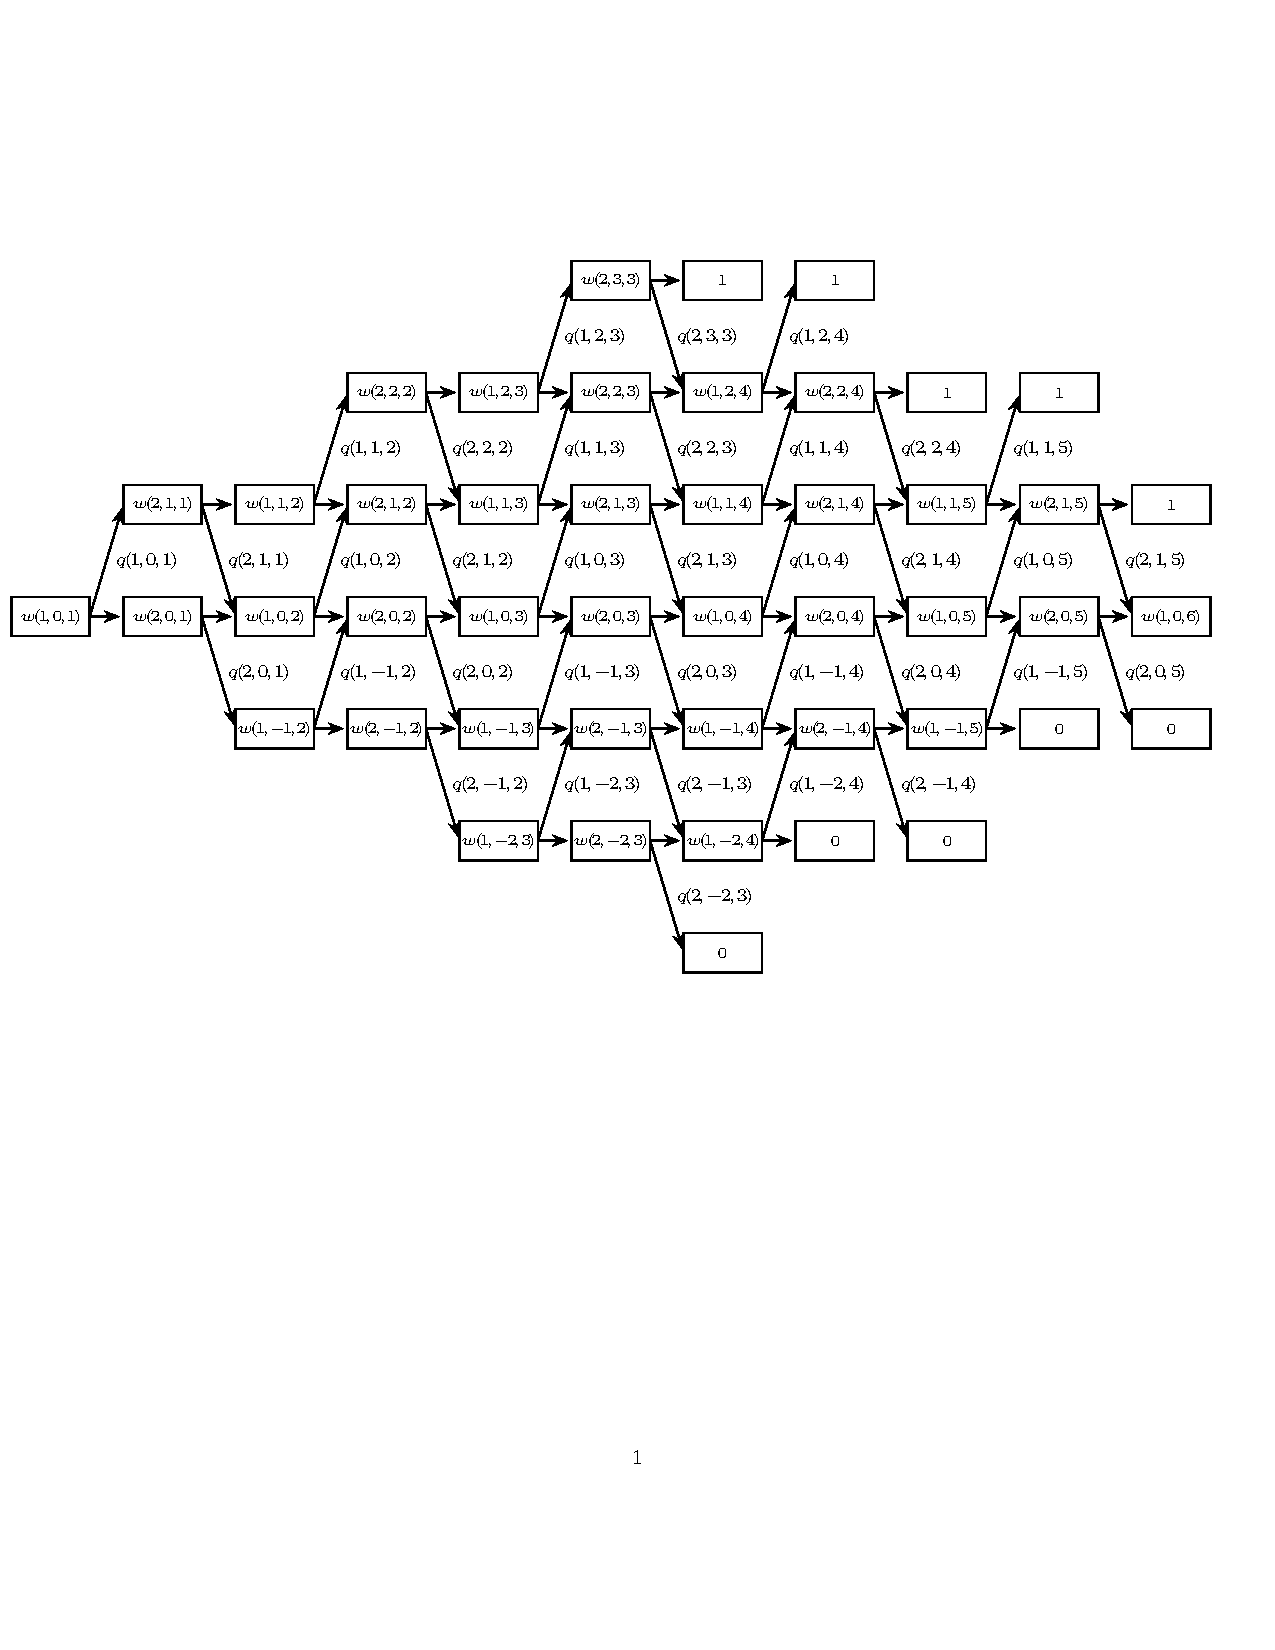
\includegraphics[clip,width=1\columnwidth]{one_shot_network_v4}\\
 \vskip-0.7in \caption{Binomial network state and transition probabilities for first 5 rounds
of penalty shootout.}
\vskip-0.4in \label{fig:BinNetwork} \vskip-0.7in 
\par\end{centering}
\vskip0.1in 
\end{figure}

Figure \ref{fig:BinNetwork} shows the different states and the corresponding
winning probabilities and transition probabilities across states.
Note that the network of states includes ending nodes with $w(k,s,t)$
equals one or zero, corresponding to the first or second team winning.
Specifically, the ending nodes are
\[
w\left(1,3,4\right)=w\left(2,3,4\right)=w\left(1,2,5\right)=w\left(2,2,5\right)=w\left(1,1,6\right)=1,
\]
and 
\[
w\left(1,-3,4\right)=w\left(2,-2,4\right)=w\left(1,-2,5\right)=w\left(2,-1,5\right)=w\left(1,-1,6\right)=0.
\]

There is one ending node with winning probability $w\left(1,0,6\right)$
different from zero and one, which represents the start of the decisive
rounds (beyond round 5). Its winning probability can be computed by
the recursion

\[
w\left(1,0,6\right)=q\left(1,0,6\right)\left(1-q\left(2,1,6\right)\right)+\left(1-q\left(1,0,6\right)\left(1-q\left(2,1,6\right)\right)-\left(1-q\left(1,0,6\right)\right)q\left(2,0,6\right)\right)w\left(1,0,6\right).
\]
Solving for $w\left(i,s,t\right)$ gives 
\[
w\left(1,0,6\right)=\frac{q\left(1,0,6\right)\left(1-q\left(2,1,6\right)\right)}{q\left(1,0,6\right)\left(1-q\left(2,1,6\right)\right)+\left(1-q\left(1,0,6\right)\right)q\left(2,0,6\right)}.
\]

The recursion equations for the remaining nodes of the network in
Figure \ref{fig:BinNetwork} are given by 
\[
w\left(k,s,t\right)=q\left(k,s,t\right)w\left(3-k,s+3-2k,t+k-1\right)+\left(q\left(k,s,t\right)\right)w\left(3-k,s,t+k-1\right).
\]

The importance of the shot taken in state $(k,s,t)$ is represented
in the change in winning probability of team $k$ calculated as:
\[
\Delta Pwin(k,s,t)=\begin{cases}
w(2,s+1,t)-w(2,s,t) & \qquad\text{ if team \ensuremath{k=1}}\\
-[w(1,s-1,t+1)-w(1,s,t+1)], & \qquad\text{ if team \ensuremath{k=2}}
\end{cases}
\]
(recall that the winning probability of the second team is $1-w(2,s,t)$,
hence the minus sign for the second case).

The main challenge in this calculation is evaluating the probability
of scoring for each state, $q(k,s,t)$. A simple approach is to set
this probability as constant and independent of the state, equal to
the average scoring probability in the overall sample (73.4\%). Another
approach is to estimate this probability based on the actual transitions
rates observed in the data, as described in the Appendix XYXY. <\textcompwordmark{}<
TO DO: calculate DeltaPwin using the scoring probabilities calculated
in the previous section and check how much it changes. My hunch is
that they are very similar. ADITYA, NILS: If we are including this,
you have to calculate DeltaPwin using these transition probabilities
and provide them in a similar format.>\textcompwordmark{}>

Alternative measures of shot importance were also considered. In some
states, missing the shot implies that the team loses or wins with
probability one. The covariate $EndIfMiss$ indicates states where
scoring lead to a terminal state where the shooting team loses\emph{;
}the covariate \emph{$EndIfScore$ }indicates shots where the shooting
team wins if it scores. It is plausible that this factor externs pressure
on the shooter. Note however that this effect applies only to states
on the outskirt of the network of Figure \ref{fig:BinNetwork}, leading
to an ending node.

Table \ref{tab:summstat_pwin} shows summary statistics of these covariates
for the shootouts in the sample. The statistics show that the consequences
of missing the shot tend to be bigger for later rounds: $\Delta Pwin$
increases (on average) as the rounds progress. Moreover, this increase
in $\Delta Pwin$ is larger for the second team after round 3. A similar
pattern is observed for the frequency of shots in which missing implies
losing the game: in the fourth round, in 20\% of the shots of the
second team lead to a loss if missed, compared to only 6\% for the
first shot in the round. The difference in the fifth round is 57\%
for the second shot vs. 29\% for the first. From rounds 3 onwards,
the consequences of the second shot in every round seem to be higher,
plausibly exerting more pressure on the shooter.

\begin{table}
\caption{Summary statistics of $\Delta Pwin$ and $EndIfMiss$\label{tab:summstat_pwin}}

\centering%
\begin{tabular}{cccccccccccc}
 & \multicolumn{3}{c}{$\Delta Pwin$} &  & \multicolumn{3}{c}{$EndIfMiss$} &  & \multicolumn{3}{c}{$EndIfScore$}\tabularnewline
\cline{2-4} \cline{6-12} 
Round & first & second & Diff &  & first & second & Diff &  & first & second & Diff\tabularnewline
\hline 
 &  &  &  &  &  &  &  &  &  &  & \tabularnewline
1 & 27.4 & 27.4 & 0.0 &  & 0.0\% & 0.0\% & 0.0\% &  & 0.0\% & 0.0\% & 0.0\%\tabularnewline
2 & 27.6 & 27.3 & -0.3 &  & 0.0\% & 0.0\% & 0.0\% &  & 0.0\% & 0.0\% & 0.0\%\tabularnewline
3 & 27.4 & 27.4 & 0.0 &  & 0.0\% & 3.5\% & 3.5\% &  & 0.0\% & 0.8\% & 0.8\%\tabularnewline
4 & 28.2 & 30.7 & 2.6 &  & 6.1\% & 20.0\% & 13.9\% &  & 8.0\% & 11.3\% & 3.3\%\tabularnewline
5 & 35.6 & 50.0 & 14.4 &  & 29.1\% & 57.1\% & 28.0\% &  & 27.9\% & 42.9\% & 15.0\%\tabularnewline
6 & 50.0 & 50.0 & 0.0 &  & 0.0\% & 73.2\% & 73.2\% &  & 0.0\% & 26.8\% & 26.8\%\tabularnewline
\hline 
\end{tabular}
\end{table}

Several specifications were estimated to measure the effect of $\Delta Pwin$,
$EndIfMiss$ and $EndIfScore$ on shooting performance. The specifications
are described in Table \ref{tab:results_deltaprob}. All the specifications
include dummy variables for round number, competition and team fixed
effects.

\begin{table}
\caption{Estimation results including proxies of pressure that account for
the consequences of the shot (for APH competitions)\label{tab:results_deltaprob}}

{
\def\sym#1{\ifmmode^{#1}\else\(^{#1}\)\fi}
\begin{tabular}{l*{3}{c}}
\hline\hline
                    &\multicolumn{1}{c}{(1)}&\multicolumn{1}{c}{(2)}&\multicolumn{1}{c}{(3)}\\
                    &\multicolumn{1}{c}{BASE2}&\multicolumn{1}{c}{EndMiss2}&\multicolumn{1}{c}{MissScore2}\\
\hline
FirstShot           &      0.0162         &      0.0130         &      0.0137         \\
                    &    (0.0162)         &    (0.0169)         &    (0.0171)         \\
[1em]
first $\times$ After2nd&      0.0439\sym{*}  &      0.0401         &      0.0311         \\
                    &    (0.0197)         &    (0.0215)         &    (0.0204)         \\
[1em]
EndIfMiss           &                     &     0.00897         &                     \\
                    &                     &    (0.0215)         &                     \\
[1em]
EndIfScore          &                     &      0.0242         &                     \\
                    &                     &    (0.0223)         &                     \\
[1em]
$\Delta Pwin$       &                     &                     &    -0.00187\sym{**} \\
                    &                     &                     &  (0.000591)         \\
\hline
Observations        &        9420         &        8823         &        8823         \\
\hline\hline
\multicolumn{4}{l}{\footnotesize Standard errors in parentheses}\\
\multicolumn{4}{l}{\footnotesize \sym{*} \(p<0.05\), \sym{**} \(p<0.01\), \sym{***} \(p<0.001\)}\\
\end{tabular}
}

\end{table}

Column (1) is the base specification identical to the last column
of table \eqref{tab:results_shotbase}, chosen as the preferred model
to describe the first shooter advantage. This base model suggests
that the first shooter advantage is significant on the 3rd and following
rounds, but statistically insignificant in the first two rounds. Specification
(2) includes the covariates $EndIfMiss$ and $EndIfScore$ to capture
shooter pressure. Both covariates have coefficients that are not statistically
different from zero. Note that the effect of first mover advantage
(the interaction term first$\times$After2nd) is smaller and with
smaller statistical significance (dropped from 0.05 to 0.1, not reported).
The specification shown in column (3) includes $\Delta Pwin$ as a
measure of pressure \textendash{} its coefficient is negative and
highly statistically significant. A 10\% increase in this probability
implies a 1.87\% decrease in the probability of scoring. Moreover,
the first mover advantage is not statistically different from zero
at any reasonable significance level. Note that Table \ref{tab:summstat_pwin}
shows that at round 5 the average difference in $\Delta Pwin$ between
the first and second team is about 14.4\%, which implies an overall
effect of $14.4\%\times0.187\%=2.7\%$. This is about half the difference
in shooting performance reported in Table \ref{tab:summstat_shot}
in the 5th round. Hence, the results suggests that the measure of
pressure $\Delta Pwin$ mediates a significant portion of the first-mover
advantage, accounting for about half of the difference in scoring
performance between first and second shooter. Moreover, the remaining
first shooter advantage after controlling for pressure is not statistically
different from zero after we account for this effect.

The same analysis was repeated with the extended sample of competitions,
reported in Appendix Table \ref{tab:results_deltaprob_ext}. The results
are similar in their direction and magnitude, and the statistical
significance of several of the coefficients increase due to the higher
precision in the estimates. The $EndIfMiss$ coefficient is positive
and becomes statistically significant in the specification of column
(2). An important change in the estimates is that the interaction
of first shot and after 2nd round indicator becomes significant in
Column (3) (this is because the estimate is more precise), suggesting
that the effect of the first mover advantage is not completely mediated
by the the pressure measure $\Delta Pwin$.

Overall, the analysis of individual shots corroborates the presence
of a first-mover advantage. The results suggests that: (1) the difference
between the first and second shooter on every round becomes more pronounced
on the 3rd round onwards; (2) an important portion of this advantage
is explained through the higher pressure that the second shooter faces
from the consequences of missing a shot, which is much higher for
the second shooter from the third round onwards. These results are
useful to simulate the impact of changing the shooting sequence, which
is analyzed in the next section.

\section{Evaluating alternative shooting sequences\label{sec:sequence}}

Although most of previous work has focused in analyzing data at the
shootout level, the analysis on the previous section shows that studying
shooter's behavior at the shot level is useful to uncover the mechanisms
that drive the first mover advantage. Doing so is critical to analyze
counterfactual scenarios of changing the shot sequence, in order to
evaluate the impact of these changes in the outcomes of the shootout.

\subsection{Modeling round transitions}

Although the decision on which team starts shooting is determined
by a ``fair coin'', the current mechanism if viewed as unfair because
it introduces an external factor (the luck of the coin) that affects
the outcome of shootout. Hence, the objective is to devise a mechanism
that minimizes this impact of these external factor so that when two
identical teams are confronted they have similar chances of winning,
regardless on how the order of the shots was determined. 

The empirical results suggest that the current shooting scheme makes
the second team face a higher pressure overall, because the impact
on the outcome of, in particular, later shots has a larger effect
on the probability of winning the match. This effect can potentially
be reduced by alternative sequencing of the teams. On this regard,
\citet{palacios2014beautiful} proposes two alternative schemes:
\begin{itemize}
\item ABBA: The team who takes the first shot goes second on even rounds
and first on odd rounds. The resulting sequence is ABBAABBA.
\item Thue-Morse sequence: this sequence takes an alternating pattern, so
that if the two beginning shots where AB, the next would take the
opposite order (or mirror image) BA, so the initial four shots are
similar to ABBA. However, the next shots take the mirror image as
the last four, BAAB, changing the pattern to ABBABAAB. The next eight
shots would be the mirror image of these, BAABABBA, and so on. The
logic behind the Thue-Morse sequencing scheme is that if a particular
order in a subsequence of shots favors one player, then taking the
mirror image in the following shots compensates by giving that advantage
to the other player.
\end{itemize}
Analyzing the performance of these alternating sequences requires
measuring how the shot performance is affected when the order of shots
is altered. Given that the sequencing of shootouts have always operated
with the same scheme, observational data is limited to study empirically
the effect of order sequencing on shot performance. An alternative
option is to run a controlled laboratory experiment to study how shot
performance is affected under different shot sequences: \citet{palacios2014beautiful}
report such experiments comparing the current scheme, ABBA and Thue-Morse
and report that the latter two reduce the first mover advantage significantly.
However, given that the driving mechanism appears to be pressure,
it is difficult to replicate the actual pressure faced by players
in a high-stakes match into the lab. The best alternative would be
to run a field experiment \textendash{} in fact, FIFA tested the ABBA
scheme for the Youth Worldcup in 2017 <\textcompwordmark{}<FIND ARTICLE
>\textcompwordmark{}>, but the small sample sizes precludes taking
conclusions on the impact of the effect.

\subsection{A network model to analyze outcomes of penalty shootouts}

The approach taken here is to use part of the empirical results from
the shot-by-shot analysis to simulate the outcome of a shootout under
alternative sequencing schemes. In doing so, the following assumptions
are made regarding the relationship between shot performance and the
shot sequences. First, the scoring probability of a penalty depends
only on the round number $t$ and the outstanding score difference
(before the shot is taken). Specifically, the score probability is:
(i) independent from the path during period $1\ldots t-1$ at which
the score difference was reached; (ii) independent on the forthcoming
sequence of shots for $t+1$. Second, the order in which a team chooses
the order of its shooters is not affected by the sequencing scheme.
This latter assumption is required in order to extrapolate the observed
performance of shooters under the current scheme into the simulation
of alternative sequences. For example, Table \ref{tab:summstats}
shows that the first round has a higher scoring performance that the
other rounds, which could be attributed to better players shooting
in the first round. The assumption is that the choice of the player
quality is independent of the sequencing.

Based on these assumptions, the evolution of a penalty shootout can
be modeled as a Markovian system, in a similar way as represented
by Figure \ref{fig:BinNetwork}, represented by a binomial network
with two possible outcomes coming out of each node. For the purpose
of analyzing alternative sequences, the states and the network can
be simplified as follows. The state is defined by the round $t$ and
the goal difference $s$ calculated as the partial score of the starting
team minus the second team (in contrast to the network represented
in Figure \ref{fig:BinNetwork}, the team kicking the shot is surpressed).
The transitions occur round by round, with three possible transitions
out of each node: the goal difference can increase by one (first team
scores and the second misses), decrease by one (first team misses
and the second scores), or remain constant (both teams miss or score).
This means that transitions are in the form of trinomial distributions
where the change in score difference from round to round is denoted
by $c\in\left\{ -1,0,1\right\} $.

Let $p_{c}\left(s,t\right)$ be the probability that the score difference
at the start of round $t+1$ is $s+c$ given that the score difference
at the start of round $t$ was $s$. The trinomial network is represented
in Figure \ref{fig:TriNetwork}. Then team A's ability to increase
the score difference in its favor in round $t$ when already being
ahead by $s$ is $p_{1}\left(s,t\right)$, and the counterpart of
team B is $p_{-1}\left(-s,t\right)$, and so on. It follows that the
relevant arcs for comparison are the pairs that form a mirror image
around the center of Figure \ref{fig:TriNetwork}.

<\textcompwordmark{}<{*}{*} NILS : 

-PLEASE REMOVE THE ``A'' SUPERSCRIPT FROM THE p's IN THE FIGURE

- WHAT ARE THE q's IN THE FIGURE? WE PREVIOUSLY DEFINED THEM AS SCORING
PROBABILITIES, SO SEEMS INCONSISTENT NOTATION HERE. I SUGGEST CHANGING
THE NOTATION IN THE FIGURE USING $v(s,t)$ AS THE CONDITIONAL WINNING
PROBABILITY {*}{*}>\textcompwordmark{}>

\begin{figure}[h]
% Requires \usepackage{graphicx}

\begin{centering}
\vskip-0.2in 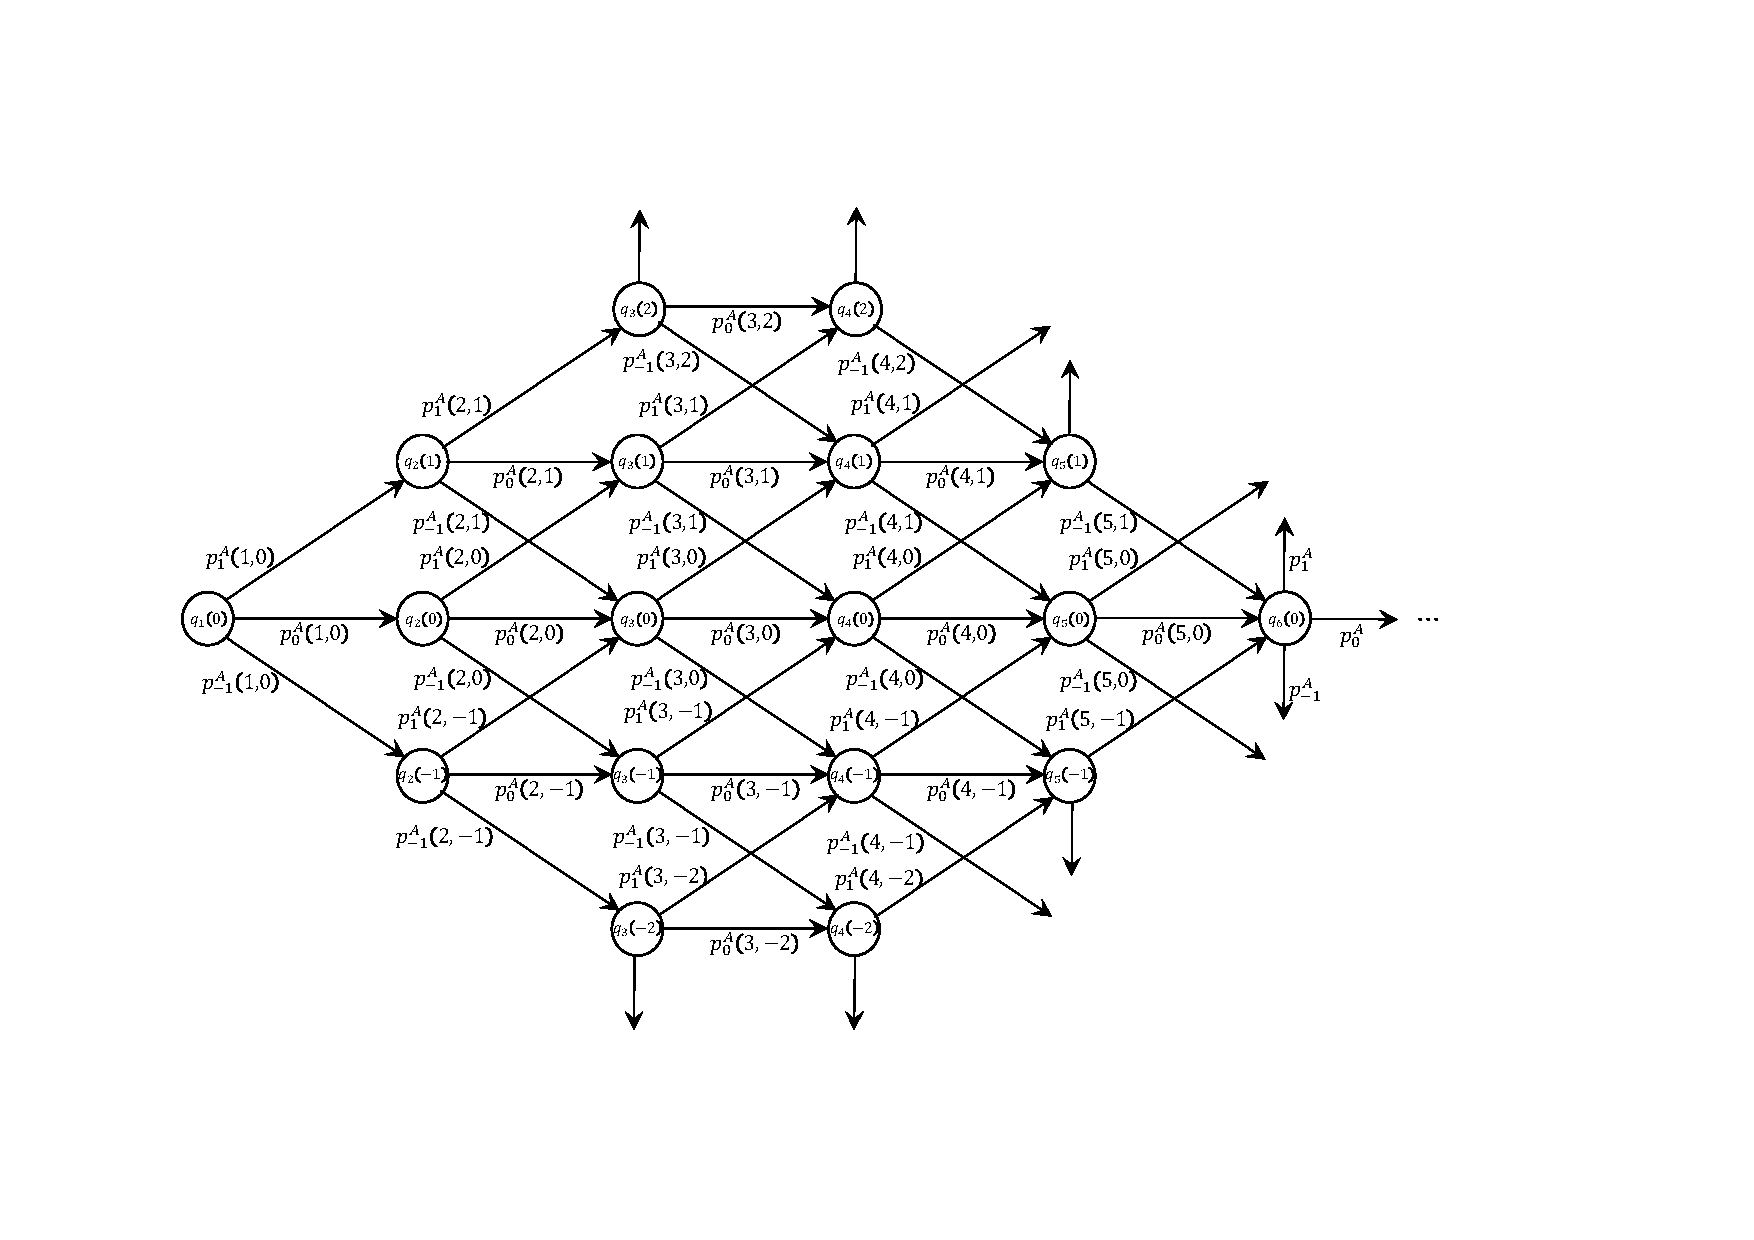
\includegraphics[clip,width=1\columnwidth]{TransitionProbs}\\
 \vskip-0.7in \caption{Trinomial network state and transition probabilities for first 5 rounds
of penalty shootout.}
\vskip-0.4in \label{fig:TriNetwork} \vskip-0.7in 
\par\end{centering}
\vskip0.1in 
\end{figure}

The first teams ability ability to increase the score difference in
its favor in round $t$ when already being ahead by $s$ is $p_{1}\left(s,t\right)$,
and the counterpart for the second team is $p_{-1}\left(-s,t\right)$.
It follows that the relevant arcs for comparison are the pairs that
form a mirror image around the center of Figure \ref{fig:TriNetwork}.
This representation of the network is sufficient to evaluate the impact
of alternative sequences, as we show next.

At each node in the network, $v\left(s,t\right)$ represents the probability
that the starting team will win the shootout out of state $\left(s,t\right)$
at the beginning of round $t$. All except one ending node of Figure
\ref{fig:TriNetwork}, namely $v\left(0,6\right)$, have values 0
or 1, i.e., 
\[
v\left(3,4\right)=v\left(2,5\right)=v\left(1,1,6\right)=1,
\]
and 
\[
v\left(-3,4\right)=v\left(-2,5\right)=v\left(-1,6\right)=0.
\]

We find $v\left(0,6\right)$ by recursion

\[
v\left(0,6\right)=p_{1}\left(0,6\right)+p_{0}\left(0,6\right)v\left(0,6\right).
\]
Solving for $v\left(s,t\right)$ gives 
\[
v\left(0,6\right)=\frac{p_{1}\left(0,6\right)}{1-p_{0}\left(0,6\right)}.
\]

The recursion equations for the remaining nodes with two outgoing
arcs of the network in Figure \ref{fig:TriNetwork} are given by:\footnote{Can also use $c=-s/|s|$ here. }
{*}{*} NILS: I WILL LET YOU DECIDE ON THE NOTATION, BUT I SUGGEST
CHOOSING ONE{*}{*}
\begin{equation}
v\left(s,t\right)=\left(1-p_{c}\left(s,t\right)\right)v\left(s,t+1\right)+p_{c}\left(s,t\right)v\left(s+c,t+1\right)\mbox{for }t\in\{4,5\},|s|=6-t,c=-sign(s)\cdot1,\label{eq:vst_2}
\end{equation}
and for the nodes with three outgoing arcs the recursion equations
are 
\begin{equation}
v\left(s,t\right)=p_{1}\left(s,t\right)v\left(s+1,t+1\right)+p_{0}\left(s,t\right)v\left(s,t+1\right)+p_{-1}\left(s,t\right)v\left(s-1,t+1\right)\mbox{for }s\in\{-2,-1,0,1,2\},t\in\{|s|+1,\ldots,5-|s|\}.\label{vst_3}
\end{equation}


\subsection{Estimating transition probabilities\label{subsec:transprob}}

The evolution of the shootout shown in Figure \ref{fig:TransProbs}
requires the transition probabilities $p_{c}(t,z)$ as primitives.
Two approaches are used to estimate these primitives. The first approach
is to gather all shots in the sample and calculate the state transitions
as sample averages from the observed transitions. This approach is
described in further detail in the Appendix.

{*}{*}{*}{*} STOPPED HERE {*}{*}{*}{*}

The second approach is parametric and considers that transitions are
generated as the outcome of two shots. The transition probabilities
$p_{c}(s,t)$ characterize the distribution of the change in the goal
difference, $c=\{-1,0,1\}.$ This underlying r.v. is the difference
of the score of the two shots in the round, $c=Y_{1}-Y_{2}$, where
$Y_{1}$ equals one when the first shot is scored, zero otherwise
(similar for the second shot $Y_{2}$). Hence, the distribution of
$c$ is uniquely determined by the distribution of $Y_{1}$ and $Y_{2}$.
Following the notation used in section \ref{subsec:deltaPwin}, the
distribution of these two r.v.s are modeled as:
\begin{itemize}
\item $q(1,s,t)$, the scoring probability of the first shot in state $(s,t)$.
\item $q_{2}(2,s+Y_{1},t)$, the scoring probability of the second shot
in state $(s,t)$ when the first shot outcome is $Y_{1}$. In some
terminal nodes the game ends before the second shot of the round is
taken. The probability $q_{2}$ is undefined for those states.
\end{itemize}
The transition probabilities for the network are given by:
\begin{eqnarray*}
p_{1}(s,t) & = & q_{1}(s,t)\times(1-q_{2}(s+1,t))\\
p_{-1}(s,t) & = & q_{2}(s,t)\times(1-q_{1}(s,t))\\
p_{0}(s,t) & = & 1-p_{1}(s,t)-p_{-1}(s,t)
\end{eqnarray*}

The shot scoring probabilities $q_{1}$ and $q_{2}$ are estimate
with a logistic regression that includes dummy variables for round
interacted with dummies for goal difference and dummies for first/second
shooter. An additional dummy variable is included in the second shot
of each round indicating if the first shot was score or miss ($Y_{1}$).
This is a saturated model that provides sufficient flexibility to
accomodate different patterns of the transition probabilities. As
additional controls, the model includes dummy variables for the type
of competition.

\subsection{Statistical tests to compare trinomial transitions}

<\textcompwordmark{}<{*}{*} NOTE MO: I DON'T UNDERSTAND WHAT THIS
ANALYSIS IS ADDING TO THE MAIN OBJETIVE OF THE PAPER. ADITYA AND NILS
, PLEASE WRITE THE MOTIVATION AND THE CONCLUSIONS FROM THIS SECTION{*}{*}>\textcompwordmark{}>

Let $\bar{p}$ denote the expected change. Specifically, for $s\geq0$,
\[
\bar{p}_{c}\left(s,t\right)=p_{1}\left(s,t\right)-p_{-1}\left(s,t\right),
\]
and 
\[
\bar{p}_{-c}\left(-s,t\right)=p_{-1}\left(-s,t\right)-p_{1}\left(-s,t\right).
\]

We here to statistical (one sided) tests using bootstrapping with
100,000 samples of the dataset.

AER competitions:

<\textcompwordmark{}<{*}{*} SOME OF THE TESTS GIVE DIFFERENT RESULTS
DEPENDING ON HOW $p_{c}(s,t)$ WAS CALCULATED. WHICH IS THE CORRECT
ESTIMATOR TO USE?? YOU CAN USE SIMULATION TO EVALUATE THE PERFORMANCE
OF THE TWO ESTIMATORS AND CHOOSE ONE{*}{*}>\textcompwordmark{}>

\begin{tabular}{c|c|c||r|r|l||r|r|l|r|}
test  & $t$  & $|s|$  & $\bar{p}_{c}\left(s,t\right)$  & $\bar{p}_{-c}\left(-s,t\right)$  & $p$-value  & $\bar{\rho}_{c}$  & $-\bar{\rho}_{-c}$  & $p$-value  & \tabularnewline
\hline 
\multirow{9}{*}{one trinomial} & 1 & 0 & 0.0074 &  & 0.3645 & 0.0074 &  & 0.3605 & \tabularnewline
 & 2 & 0 & 0.0001 &  & 0.5116 & {-}0.0077 &  & 0.6298 & \tabularnewline
 & 3 & 0 & 0.0272 &  & 0.1859 & 0.0508 &  & 0.0325{*} & \tabularnewline
 & 4 & 0 & 0.0373 &  & 0.1480 & 0.0145 &  & 0.3218 & \tabularnewline
 & 5 & 0 & 0.1100 &  & 0.0022{*}{*} & 0.1092 &  & 0.0009{*}{*}{*} & \tabularnewline
 & 6 & 0 & 0.0270 &  & 0.1706 & 0.0270 &  & 0.1666 & \tabularnewline
 &  & 0 & 0.0348 &  & 0.0024{*}{*} & 0.0335 &  & 0.0018{*}{*} & \tabularnewline
\hline 
\multirow{5}{*}{two trinomials} & 2 & 1 & 0.1002 & 0.0861 & 0.4190 & 0.0959 & 0.0530 & 0.2547 & \tabularnewline
 & 3 & 1 & 0.0632 & {-}0.0538 & 0.0270{*} & 0.0167 & {-}0.0269 & 0.2161 & \tabularnewline
 & 4 & 1 & 0.0221 & {-}0.0140 & 0.2842 & 0.0535 & {-}0.0181 & 0.1038 & \tabularnewline
 & 3 & 2 & {-}0.0230 & {-}0.0766 & 0.3460 & 0.0054 & {-}0.1664 & 0.0769. & \tabularnewline
 &  & 1 & 0.0618 & 0.0061 & 0.0657. & 0.0554 & 0.0027 & 0.0650. & \tabularnewline
\hline 
\multirow{2}{*}{two binomials} & 4 & 2 & {-}0.0564 & {-}0.1694 & 0.0204{*} & {-}0.0725 & {-}0.1881 & 0.0030{*}{*} & \tabularnewline
 & 5 & 1 & {-}0.1600 & {-}0.1748 & 0.3456 & {-}0.1609 & {-}0.1768 & 0.3007 & \tabularnewline
\hline 
\end{tabular}

Some comments about these tests: It seems like the comparison of two
trinomials is not as sharp as it could be as it does not utilize the
ordinal nature of the transitions. $<$NR: ref. earlier discussions
and notes. Could one possibility be to do some kind of likelihood
test?$>$

For the comparison of two binomials, the expected value of transition
is misleading in this table. $<$NR: should we do this in separate
table?$>$ The expected values are the value of the arc going towards
the centre of the network.

<\textcompwordmark{}< ADITYA, NILS: SOME CONCLUSIONS NEED TO BE ADDED
HERE >\textcompwordmark{}>

\subsection{Calculation of winning probabilities for alternative shot sequences}

The structure of the trinomial network (Figure \ref{fig:TriNetwork})
and the estimated parameters can be used to analyze the outcome of
alternative sequence schemes, specifically ABBA and Thue-Morse (TM).
For notation, Team A refers to the team that takes the first shot
in the first round, and Team B the second shot. 

A sequence scheme is defined by the vector $\gamma=\left(\gamma_{1},\gamma_{2},\gamma_{3},\ldots\right)$
that define the team that take the first shot in every round $t$.
Define $\gamma_{t}=1$ when team A goes first in round $t$ (by definition,
$\gamma_{1}=1$) and $\gamma_{t}=-1$ if team B goes first in round
$t$. The evolution of the penalty shootout under sequence scheme
$\gamma$ is defined by adjusting the transition probabilites of the
trinomial network so that $\tilde{p}_{c}\left(s,t\right)=p_{\gamma_{t}c}\left(\gamma_{t}s,t\right)$.

To calculate the conditional winning probabilities $v(s,t)$ for the
TM sequence, we compute $v^{TM}\left(0,6\right)$ by doing the recursion
until convergence <\textcompwordmark{}< {*}{*}{*} THE LAST STATEMENT
IS NOT CLEAR {*}{*}>\textcompwordmark{}>, while for ABBA we get the
probability that team A will win the shootout, conditioned of it being
extended past the initial 5 rounds, by the recursion:

<\textcompwordmark{}<{*}{*} SHOULD ALL THE p's BELOW HAVE TILDE?{*}{*}>\textcompwordmark{}>

\[
v^{ABBA}\left(0,6\right)=p_{-1}\left(0,6\right)+p_{0}\left(0,6\right)\left(p_{1}\left(0,6\right)+p_{0}\left(0,6\right)v^{ABBA}\left(0,6\right)\right).
\]
Solving for $v^{ABBA}\left(0,6\right)$ gives 
\begin{eqnarray*}
v^{ABBA}\left(0,6\right) & = & \frac{p_{-1}\left(0,6\right)+p_{0}\left(0,6\right)p_{1}\left(0,6\right)}{1-p_{0}^{2}\left(0,6\right)}\\
 & = & \frac{\left(1-p_{0}\left(0,6\right)-p_{1}\left(0,6\right)\right)+p_{0}\left(0,6\right)p_{1}\left(0,6\right)}{\left(1-p_{0}\left(0,6\right)\right)\left(1+p_{0}\left(0,6\right)\right)}\\
 & = & \frac{1-p_{1}\left(0,6\right)}{1+p_{0}\left(0,6\right)}.
\end{eqnarray*}

All the remaining transitions can be calculated using equations (\ref{eq:vst_2})
and (\ref{vst_3}) replacing $p_{c}(s,t)$ by the adjusted transition
$\tilde{p}_{c}(s,t)$.

\subsection{Hypothesis testing}

The main objective of this analysis is to evaluate whether alternative
sequencing schemes can help in reducing the gap in the winning probability
between the team that take the first shot and other team. Based on
Figure \ref{fig:TriNetwork}, denote by $W^{ABAB}=v_{1}^{ABAB}(0)$
, $W^{ABBA}=v_{1}^{ABBA}(0)$ and $W^{TM}=v_{1}^{TM}(0)$ the winning
probabilities of the starting team under the current, ABBA and Thue-Morse
sequencing schemes, respectively. We seek to compare these winning
probabilities and test whether the alternative schemes ABBA and Thue-Morse
help to reduce the first mover advantage. Specifically, the following
pairwise hypothesis tests are evaluated:
\begin{itemize}
\item Test 1: $H_{0}:\:W^{ABAB}=W^{ABBA}$ versus the alternative $H_{A}:W^{curr}>W^{ABBA}$
\item Test 2: $H_{0}:\:W^{ABAB}=W^{TM}$ versus the alternative $H_{A}:W^{curr}>W^{TM}$
\item Test 3: $H_{0}:\:W^{TM}=W^{ABBA}$ versus the alternative $H_{A}:W^{TM}<W^{ABBA}$
\end{itemize}
Rejecting the Null implies that one of the schemes reduces the first
mover advantage. In addition, it is of interest to test if a first
mover advantage prevails under each of the alternative sequence schemes:
\begin{itemize}
\item Test 4: $H_{0}:\:W^{ABAB}=0.5$ versus the alternative $H_{A}:W^{ABAB}>0.5$
\item Test 5: $H_{0}:\:W^{ABBA}=0.5$ versus the alternative $H_{A}:W^{ABBA}>0.5$
\item Test 6: $H_{0}:\:W^{TM}=0.5$ versus the alternative $H_{A}:W^{TM}>0.5$
\end{itemize}
Failing to reject the Null implies that the sequence scheme was effective
in eliminating the first mover advantage.

These hypothesis test can be conducted with a point estimate of $W$
and its corresponding confidence interval. A valid point estimate
fo can be obtained by first estimating the transition probabilities
$p_{x}(t,z)$ using one of the methods described in Section \ref{subsec:transprob}.
Using these estimates, compute the estimate of $W$ via recursion,
using the corresponding sequencing schemes (using the recursion for
each sequence scheme described in the previous section). The challenge
is to construct a confidence interval for this point estimate. Although
the confidence intervals of the transition probabilities $p_{x}(t,z)$
can be computed through standard methods (i.e. asymptotic confidence
intervals), the estimators $\hat{W}$ are a convoluted function of
the transition probabilities and therefore its standard error and
asymptotic distribution is difficult to compute.

Bootstrapping provides a feasible approach to conduct these hypothesis
tests. The main idea of bootstrapping is to compute the distribution
of the estimators $\hat{p}$ and $\hat{W}$ by simulating the sampling
process behind the estimation. The sampling process is a follows:
(1) sample $n$ \emph{shootouts} from a population of matches; (2)
using the sample of shootouts and its corresponding shots round-by-round,
estimate the transition probabilities $\hat{p}_{x}(t,z)$ through
some method (parametric or non-parametric). (3) Compute $\hat{W}$
using the estimates $\hat{p}_{c}(t,z)$ through recursion (using the
corresponding sequence scheme).

The following algorith is used to construct the confidence interval
of the estimator $\hat{W}$:
\begin{enumerate}
\item Take a re-sample of size $n$ (with replacement) from the original
sample of matches (some matches could get repeated). Denote the shootouts
in this resample $S_{r}$ (the subscript indexes the resample)
\item Using the resample $S_{r}$, estimate $\hat{p}^{(r)}$ (for all states
$(s,t)$ and $c\in\{-1,0,1\}$).
\item Compute the estimator $\hat{W}^{(r)}$ using the estimated $\hat{p^{(r)}}$,
for each sequencing schemes.
\item Store the estimates of the current run, $\hat{W}^{(r)}=(\hat{W}^{curr,(r)},\hat{W}^{ABBA,(r)},\hat{W}^{TM,(r)})$.
Repeat to take a new resample $s+1$.
\item Iterate for many (e.g. $R=1000)$ resamples.
\end{enumerate}
The point estimates $\{\hat{p}^{(s)}\}_{s}$ and $\{\hat{W}^{(s)}\}_{s}$
provide an empirical distribution of the estimators $\hat{p}_{x}(t,z)$
and $(\hat{W}^{curr},\hat{W}^{ABBA},\hat{W}^{TM})$. 

Two estimators are constructed, the first using the non-parametric
estimates of the trinomial transitions (estimates reported in Table
\ref{tab:Westim_nonparm})and the second using the parametric estimates
(reported in Table \ref{tab:Westim_param}). In general, both estimators
provide similar results. As expected, the current sequencing ABAB
gives the largest point estimate, slightly above 54\%, similar to
the first mover advantage estimated in section \ref{sec:data}. The
99\% confidence interval is {[}50.7, 58.32{]}), which does not contain
the Null value 50\%, therefore Test 4 is rejected at the 1\% significance
level. These results are consistent with those obtained with the shootout
level analysis described in section \ref{sec:data}, both in terms
of magnitude and statistical significance of the first mover advantange
in the ABAB sequence scheme. 

For the ABBA scheme, both estimators give smaller point estimates
of the winning probability, close to 50\%. The 99\% confidence interval
contains 50\%, therefore Test 5 cannot be rejected. However, it is
rejected at the 5\% significance level, providing some evidence that
ABBA does not fully eliminate the first mover advantage. For Thue-Morse,
the point estimate is even smaller, and both the 99\% and 95\% confidence
interval also contains 50\%, failing to reject Test 6. Overall, the
estimates predict that for ABBA and Thue-Morse the first mover advantage
is smaller, and in Thue-Morse both teams have equal probabilities
of winning .

\begin{table}
\centering%
\begin{tabular}{crrrrrr}
\hline 
sequence  & average  & 0.01  & 0.05  & 0.50  & 0.95  & 0.99 \tabularnewline
\hline 
ABAB  & 0.5456  & 0.5070  & 0.5188  & 0.5456  & 0.5725  & 0.5832 \tabularnewline
ABBA  & 0.5250  & 0.4908  & 0.5010  & 0.5250  & 0.5491  & 0.5591 \tabularnewline
T-M  & 0.4805  & 0.4465  & 0.4564  & 0.4805  & 0.5045  & 0.5142 \tabularnewline
\hline 
\end{tabular}

\caption{Bootstrap distribution of the estimator of winning probabilities of
the starting team, under three different possible shot sequences,
using \textbf{non-parametric} estimator of the trinomial transition
probabilities $p_{c}(s,t)$. \label{tab:Westim_nonparm}}
\end{table}

\begin{table}
{*}{*} NILS, ADITYA: Please add the additional percentiles to this
table so that it looks similar to the previous one {*}{*}

\centering%
\begin{tabular}{ccccc}
\cline{1-4} 
Sequence & mean & p1 & p5 & \tabularnewline
\cline{1-4} 
Current & 0.5472 & 0.5172 & 0.5260 & \tabularnewline
ABBA & 0.5050 & 0.4998 & 0.5013 & \tabularnewline
Thue-Morse & 0.4972 & 0.4919 & 0.4939 & \tabularnewline
\cline{1-4} 
\end{tabular}

\caption{Bootstrap distribution of the estimator of winning probabilities of
the starting team, under three different possible shot sequences,
using \textbf{parametric} estimator of the trinomial transition probabilities
$p_{c}(s,t)$. \label{tab:Westim_param}}
\end{table}

To conduct the pairwise Test 1, the statistic $t^{(r)}=\hat{W}^{curr,(r)}-\hat{W}^{ABBA,(r)}$
is computed for each bootstrapped sample $r$. The Null hypothesis
$W^{ABAB}=W^{ABBA}$ is rejected at the $\alpha$ significance level
if the $\alpha$ bottom percentile of the sample $t^{(r)}$ is greater
than zero (one-sided test). A similar test can be conducted for Test
2 and 3. Table \ref{tab:pairwise_param} report the results for these
tests. The difference in winning probability of ABAB and ABBA is positive
and statistically significant at the 1\% level. Similar results is
obtained for the difference between ABAB and Thue-Morse sequences.
Overall, Test 1 and 2 suggest that the probability of winning of the
starting team is significantly (statistically) greater under the current
sequence scheme relative to ABBA or Thue-Morse. The difference is
in the order of 4-5\% reduction for the alternative schemes. In contrast,
the results suggest that ABBA and Thue-Morse have about the same winning
probability for the starting team, with a difference in probability
less than 0.8\% (ABBA is slightly greater). The 99\% confidence interval
of the difference contains the Null value zero, indicating that the
Null of equal winning probabilities cannot be rejected at that significance
level; it is though rejected at the 5\% significance level. In any
case, the difference appears to be much smaller relative to the difference
with respect to the current scheme.

{*}{*} NILS, ADITYA: Please add similar calculations of the Table
below using the non-parametric estimates {*}{*}

\begin{table}
\centering%
\begin{tabular}{ccccccc}
\hline 
 &  & mean & p1 & p5 & p95 & p99\tabularnewline
\hline 
Test 1 & ABAB- ABBA & 0.0422 & 0.0154 & 0.0234 & 0.0612 & 0.0682\tabularnewline
Test 2 & ABAB - TM & 0.0499 & 0.0168 & 0.0276 & 0.0718 & 0.0826\tabularnewline
Test 3 & ABBA - TM & 0.0077 & -0.0017 & 0.0011 & 0.0149 & 0.0183\tabularnewline
\end{tabular}

\caption{Boostrap distribution of the differences in winning probabilities
between alternative sequence mechanisms, based on parametric estimators
of $p_{c}(s,t)$ \label{tab:pairwise_param}}
\end{table}

Overall, the counterfactual simulations analyzed in this section suggest
that the first mover advantage can be significantly reduced under
the alternative sequencing of shoots studied, both ABBA and Thue-Morse.
The advantage of Thue-Morse over ABBA appears to be very small. Given
the simplicity of ABBA, which is also used in other sports such as
tie-break in Tennis, it seems to be a preferable sequence scheme to
reduce the effect of external factors on the outcome of the shootout.

\section{Conclusions\label{sec:conclusions}}

The main conclusions so far:

- We find a first mover advantage in penalty shootouts, based on an
expanded dataset including the same competitions as previous work
and also expanding to other competitions.

- We conduct a detailed analysis shot-by-shot to uncover the underlying
mechanism that drives the first mover advantage. We construct a measure
of pyschological pressure that explains most of the first mover advantage.

- We conduct simulations, calibrated with the observed data, to estimate
the effect of alternative sequence schemes on the winning probability
of the starting team. These simulations show that using a simple scheme
such as ABBA reduces significantly the winning probability of the
first team.

- More complicated sequence schemes such as Thue-Morse, have marginal
impact in reducing the first mover advantage relative to ABBA, but
in the simulations it appears as fully eliminating the first mover
advantage.

\bibliographystyle{\string"../../engagement paper/lyx/ormsv080\string"}
\bibliography{penalties_biblio}

\pagebreak{}

\appendix

\section{Estimation of scoring probabilities using state transitions}

Let $n_{x}=\sum_{i=1}^{n}\mathbf{1}_{x_{j}}$ be a counter function
of the number of shootouts that for shootout $i$ satisfy the logical
test $x_{i}$. Let $\left(k,s_{1},s_{2},t\right)_{i}$ be true if
and only if shootout $i$ travels the path involving that team $k$'s
shot makes the score difference change from $s_{1}$ to $s_{2}$ in
round $t$. Then $n_{k,s,s,t}$ denote the number of shots taken by
team $k$ in round $t$ that is missed (i.e., it goes from score difference
$s$ to the same score difference $s$), and let $n_{k,s,s+3-2k,t}$
denote the shots taken by team $i$ in round $t$ that is scored (i.e.,
it goes from score difference $s$ and to score difference $s+1$
if team $k=1$ and to score difference $s-1$ if team $k=2$).

{*}{*} NOTATION BELOW NEEDS TO BE CHANGED. Index j -> i , index i
-> k {*}{*}

Let $q\left(i,s,t\right)$ be the probability that team $i$ score
in round $t$ from a score difference of $s$. From the data, this
is estimated by the relevant proportion

\[
\hat{q}\left(i,s,t\right)=\frac{n_{i,s,s+3-2i,t}}{n_{i,s,s,t}+n_{i,s,s+3-2i,t}},t=1,\ldots,5.
\]

For $t=6,\ldots$ we assume that the scoring probabilities are independent
of the round and us $6$ as the round number, which gives

\begin{eqnarray*}
\hat{q}\left(1,0,6\right) & = & \frac{n_{1,0,1,t}}{n_{1,0,0,t}+n_{1,0,1,t}},\\
\hat{q}\left(2,s,6\right) & = & \frac{n_{2,s,s-1,t}}{n_{2,s,s,t}+n_{2,s,s-1,t}},t=6,\ldots.
\end{eqnarray*}

When dropping an argument of a function, it represents the overall
value across all values of this argument. For example, $q\left(i,s\right)$
would mean the scoring probability of team $i$ when the score difference
is $s$ taken across all rounds $t$.

<\textcompwordmark{}< TO BE COMPLETED BY NILS AND ADITYA>\textcompwordmark{}>

\section{Estimation of transition probabilities for the Trinomial Network}

When estimating $p$, there are two alternatives. The one that may
come first to mind is using only data from shootouts that have score
difference $s$ at the start of round $t$, which gives

\begin{eqnarray*}
\hat{p}_{1}\left(s,t\right) & = & \frac{n_{1,s,s+1,t}}{n_{1,s,s,t}+n_{1,s,s+1,t}}\cdot\frac{n_{1,s,s+1,t\wedge2,s+1,s+1,t}}{n_{2,s+1,s+1,t}+n_{2,s+1,s,t}},\\
\hat{p}_{0}\left(s,t\right) & = & \frac{n_{1,s,s+1,t}}{n_{1,s,s,t}+n_{1,s,s+1,t}}\cdot\frac{n_{1,s,s+1,t\wedge2,s+1,s,t}}{n_{2,s+1,s+1,t}+n_{2,s+1,s,t}}+\frac{n_{1,s,s,t}}{n_{1,s,s,t}+n_{1,s,s+1,t}}\cdot\frac{n_{1,s,s,t\wedge2,s,s,t}}{n_{2,s,s,t}+n_{2,s,s-1,t}},\\
\hat{p}_{-1}\left(s,t\right) & = & \frac{n_{1,s,s,t}}{n_{1,s,s,t}+n_{1,s,s+1,t}}\cdot\frac{n_{1,s,s,t\wedge2,s,s-1,t}}{n_{2,s,s,t}+n_{2,s,s-1,t}}.
\end{eqnarray*}

<\textcompwordmark{}<{*}{*} NOTE MO: In the text, given that the results
are exactly the same using both methods, I decided to remove the results
of $\rho$ to simplify the reading. Below is the discussion and proposition
supporting this.>\textcompwordmark{}>

But by second thought, based on the markovian argument, notice that
for $t=2,3,4,5$ there is a second branch leading into the state $2,s+1,t$,
namely $n_{1,s+1,s+1,t}$. And, similarly, there is a second branch
leading into state $2,s,t$, namely $n_{1,s-1,s,t}$. This gives the
following estimates of the trinomial probabilities (we use $\rho$
here instead of $p$ for these estimates):

\begin{eqnarray*}
\hat{\rho}_{1}\left(s,t\right) & = & \frac{n_{1,s,s+1,t}}{n_{1,s,s,t}+n_{1,s,s+1,t}}\cdot\frac{n_{2,s+1,s+1,t}}{n_{2,s+1,s+1,t}+n_{2,s+1,s,t}},\\
\hat{\rho}_{0}\left(s,t\right) & = & \frac{n_{1,s,s+1,t}}{n_{1,s,s,t}+n_{1,s,s+1,t}}\cdot\frac{n_{2,s+1,s,t}}{n_{2,s+1,s+1,t}+n_{2,s+1,s,t}}+\frac{n_{1,s,s,t}}{n_{1,s,s,t}+n_{1,s,s+1,t}}\cdot\frac{n_{2,s,s,t}}{n_{2,s,s,t}+n_{2,s,s-1,t}},\\
\hat{\rho}_{-1}\left(s,t\right) & = & \frac{n_{1,s,s,t}}{n_{1,s,s,t}+n_{1,s,s+1,t}}\cdot\frac{n_{2,s,s-1,t}}{n_{2,s,s,t}+n_{2,s,s-1,t}}.
\end{eqnarray*}

Out initial motivation of also considering $\rho$ as an alternative
way to estimate the trinomial transition probabilities was to check
if the results of the recursions (and alternative sequences) were
robust in terms of the two alternatives. But as the following proposition
establish, for the recursions used to calculate the conditional winning
probabilities $v(s,t)$, the two alternative estimations actually
gives the same results.

\begin{proposition} The two estimators of $v\left(s,t\right)$, the
conditional winning probability of the first team in round $t$ with
goal difference $s$, that result from using the estimators $\hat{p}$
and $\hat{\rho}$ of the transition probabilities $p_{c}(s,t)$ yield
identical estimates. \end{proposition}

P{\scriptsize{}ROOF}: We will prove this result using forward recursion.
Let $m_{p}\left(s,t\right)$ and $m_{\rho}\left(s,t\right)$ be the
number of shootouts that visits state $\left(s,t\right)$ based on
the $p$ and $\rho$ transition probabilities, respectively. The starting
node is given the total number of shootouts $m_{p}\left(0,1\right)=m_{\rho}\left(0,1\right)=J$.
Since the expressions are the same, we state the recursions only based
on the $p$ transition probabilities. For nodes with only one incoming
arc, 
\[
m_{p}\left(s,t\right)=p_{c}\left(s-c,t-1\right)m_{p}\left(s-c,t-1\right).
\]
For nodes with two incoming arcs: 
\[
m_{p}\left(s,t\right)=p_{c}\left(s-c,t-1\right)m_{p}\left(s-c,t-1\right)+p_{0}\left(s,t-1\right)m_{p}\left(s,t-1\right).
\]
For nodes with three incoming arcs: 
\[
m_{p}\left(s,t\right)=p_{1}\left(s-1,t-1\right)m_{p}\left(s-1,t-1\right)+p_{0}\left(s,t-1\right)m_{p}\left(s,t-1\right)+p_{-1}\left(s+1,t-1\right)m_{p}\left(s+1,t-1\right).
\]
For proving the proposition, it is sufficient to establish that the
number of shootouts flowing through each of the states are the same
for both sets of trinomial transitions, i.e., $m_{p}\left(s,t\right)=m_{\rho}\left(s,t\right)$
for all states $\left(s,t\right)$.

First note that for the transition probabilities in round 1 and in
rounds 6+ are equal, i.e., $p_{c}\left(0,1\right)=\rho_{c}\left(0,1\right)$
and $p_{c}\left(0,6\right)=\rho_{c}\left(0,6\right)$.

We then consider the transition from round $t$ to $t+1$. For notational
convenience, we drop the round indicator $t$ for the $n$-notation
and also define $n_{2,s,\cdot}^{0}=n_{1,s,s\wedge2,s,\cdot}$ and
$n_{2,s,\cdot}^{+}=n_{1,s-1,s\wedge2,s,\cdot}$. Also let $n_{1,s}$
be the number of shootouts that started the round (dropping $t$)
at score difference $s$.

For trinomial nodes with only one incoming arc this is obvious. We
will first show that the results hold for a node with two incoming
arcs. We have

\begin{eqnarray*}
m_{p}\left(s,t+1\right)=m_{p}\left(s,t\right)\left[\frac{n_{1,s,s+1}}{n_{1,s}}\cdot\frac{n_{2,s+1,s}}{n_{1,s,s+1}}+\frac{n_{1,s,s}}{n_{1,s}}\cdot\frac{n_{2,s,s}^{0}}{n_{1,s,s}}\right]+m_{p}\left(s-1,t\right)\frac{n_{1,s-1,s}}{n_{1,s-1}}\cdot\frac{n_{2,s,s}^{+}}{n_{1,s-1,s}},
\end{eqnarray*}
and 
\begin{eqnarray*}
m_{\rho}\left(s,t+1\right) & = & m_{\rho}\left(s,t\right)\left[\frac{n_{1,s,s+1}}{n_{1,s}}\cdot\frac{n_{2,s+1,s}}{n_{1,s,s+1}}+\frac{n_{1,s,s}}{n_{1,s}}\cdot\frac{n_{2,s,s}^{0}+n_{2,s,s}^{+}}{n_{1,s,s}+n_{1,s-1,s}}\right]\\
 &  & +m_{\rho}\left(s-1,t\right)\frac{n_{1,s-1,s}}{n_{1,s-1}}\cdot\frac{n_{2,s,s}^{0}+n_{2,s,s}^{+}}{n_{1,s,s}+n_{1,s-1,s}}.
\end{eqnarray*}
Assume that $m_{p}\left(s,t\right)=m_{\rho}\left(s,t\right)=n_{1,s}$
and $m_{p}\left(s-1,t\right)=m_{\rho}\left(s-1,t\right)=n_{1,s-1}$.
Then it would follow that $m_{p}\left(s,t+1\right)=m_{\rho}\left(s,t+1\right)=n_{2,s+1,s}+n_{2,s,s}^{0}+n_{2,s,s}^{+}$.
For three incoming arcs: 
\begin{eqnarray*}
m_{p}\left(s,t+1\right) & = & m_{p}\left(s+1,t\right)\frac{n_{1,s+1,s+1}}{n_{1,s+1}}\cdot\frac{n_{2,s+1,s}^{0}}{n_{1,s+1,s+1}}+m_{p}\left(s,t\right)\left[\frac{n_{1,s,s+1}}{n_{1,s}}\cdot\frac{n_{2,s+1,s}^{+}}{n_{1,s,s+1}}+\frac{n_{1,s,s}}{n_{1,s}}\cdot\frac{n_{2,s,s}^{0}}{n_{1,s,s}}\right]\\
 &  & +m_{p}\left(s-1,t\right)\frac{n_{1,s-1,s}}{n_{1,s-1}}\cdot\frac{n_{2,s,s}^{+}}{n_{1,s-1,s}},
\end{eqnarray*}
and 
\begin{eqnarray*}
m_{\rho}\left(s,t+1\right) & = & m_{\rho}\left(s+1,t\right)\frac{n_{1,s+1,s+1}}{n_{1,s+1}}\cdot\frac{n_{2,s+1,s}^{0}+n_{2,s+1,s}^{+}}{n_{1,s+1,s+1}}\\
 &  & +m_{\rho}\left(s,t\right)\left[\frac{n_{1,s,s+1}}{n_{1,s}}\cdot\frac{n_{2,s+1,s}^{0}}{n_{1,s,s+1}+n_{2,s+1,s}^{+}}{n_{1,s+1,s+1}+n_{1,s,s+1}}+\frac{n_{1,s,s}}{n_{1,s}}\cdot\frac{n_{2,s,s}^{0}+n_{2,s,s}^{+}}{n_{1,s,s}+n_{1,s-1,s}}\right]\\
 &  & +m_{\rho}\left(s-1,t\right)\frac{n_{1,s-1,s}}{n_{1,s-1}}\cdot\frac{n_{2,s,s}^{0}+n_{2,s,s}^{+}}{n_{1,s,s}+n_{1,s-1,s}}.
\end{eqnarray*}
Assume that $m_{p}\left(s+1,t\right)=m_{\rho}\left(s+1,t\right)=n_{1,s+1}$,
$m_{p}\left(s,t\right)=m_{\rho}\left(s,t\right)=n_{1,s}$ and $m_{p}\left(s-1,t\right)=m_{\rho}\left(s-1,t\right)=n_{1,s-1}$.
Then it would follow that $m_{p}\left(s,t+1\right)=m_{\rho}\left(s,t+1\right)=n_{2,s+1,s}^{0}+n_{2,s+1,s}^{+}+n_{2,s,s}^{0}+n_{2,s,s}^{+}$.

For $t=2$ the result follows directly. By induction, it follows for
the rest of the network. $\Box$

Given this result, the estimator $\hat{p}_{c}(s,t)$ is used as the
non-parametric estimator of the transition probabilities.

\section{Additional specifications}

\begin{table}
\caption{Additional specifications for the shot-by-shot analysis, without including
team Fixed Effects}

\include{results_aer/results_shotbyshot_noFE}
\end{table}

\begin{table}
\caption{Estimation results of goal difference without Team Fixed Effects\label{tab:results_goaldif_noFE}}

\centering\include{results_aer/results_goalDif_noFE}
\end{table}


\subsection{Expanded set of competitions}

\begin{table}
\begin{tabular}{llllllll}
1 & Friendlies & 21 & Svenska Cupen & 41 & Campionato & 61 & Pokal Slovenije\tabularnewline
2 & Coupe de France & 22 & A-League & 42 & Steypakappingin & 62 & AFC Champions League Quali.\tabularnewline
3 & Kubok & 23 & Primera Divisi�n & 43 & Kup Crne Gore & 63 & Copa MX\tabularnewline
4 & Coppa Italia & 24 & Puchar Polski & 44 & Playoff & 64 & Gold Cup Quali.\tabularnewline
5 & �FB-Cup & 25 & Coupe & 45 & Football League Trophy & 65 & Major League Soccer\tabularnewline
6 & Ta�a & 26 & Cupa Romaniei & 46 & Supercup & 66 & FAI Cup\tabularnewline
7 & Copa Argentina & 27 & Welsh Cup & 47 & Irish Cup & 67 & Club World Cup\tabularnewline
8 & Cup & 28 & Ta�a da Liga & 48 & Challenge Cup & 68 & Lengjubikarinn\tabularnewline
9 & Poh�r FA\v{C}R & 29 & CAF Champions League & 49 & FFA Cup & 69 & Superkubok\tabularnewline
10 & Coupe de la Ligue & 30 & Nogometni Kup & 50 & Primera A &  & \tabularnewline
11 & Copa Libertadores & 31 & Bikar & 51 & UI-Cup &  & \tabularnewline
12 & Kypello Elladas & 32 & Suomen Cup & 52 & Cupa Moldova &  & \tabularnewline
13 & KNVB beker & 33 & Copa Conmebol & 53 & AFC Cup &  & \tabularnewline
14 & Cupen & 34 & Kup BiH & 54 & Liigacup &  & \tabularnewline
15 & T�rkiye Kupasi & 35 & Kupa & 55 & Super Cup &  & \tabularnewline
16 & Slovensky Pohar & 36 & Eesti Karikas & 56 & Copa do Brasil &  & \tabularnewline
17 & Kup Srbije & 37 & Magyar Kupa & 57 & Emperor's Cup &  & \tabularnewline
18 & Beker van Belgi� & 38 & Kup na Makedonija & 58 & Relegation &  & \tabularnewline
19 & Copa Sudamericana & 39 & State Cup & 59 & David Kipiani Cup &  & \tabularnewline
20 & DBU Pokalen & 40 & Africa Cup Qual. & 60 & Latvijas kauss &  & \tabularnewline
\end{tabular}

\caption{Additional competitions in the extended dataset\label{tab:add_comp}}
\end{table}

\begin{table}
{
\def\sym#1{\ifmmode^{#1}\else\(^{#1}\)\fi}
\begin{tabular}{l*{2}{c}}
\hline\hline
                    &\multicolumn{1}{c}{(1)}&\multicolumn{1}{c}{(2)}\\
                    &\multicolumn{1}{c}{WinH}&\multicolumn{1}{c}{WinHpre2003}\\
\hline
FirstShot           &       0.125\sym{***}&       0.211\sym{***}\\
                    &    (0.0253)         &    (0.0447)         \\
\hline
Observations        &        1698         &         534         \\
\hline\hline
\multicolumn{3}{l}{\footnotesize Robust standard errors. Includes dummies for competition and year}\\
\multicolumn{3}{l}{\footnotesize \sym{*} \(p<0.05\), \sym{**} \(p<0.01\), \sym{***} \(p<0.001\)}\\
\end{tabular}
}


\caption{Estimation results for Linear Probability Model using extended set
of competitions \label{tab:results_LPM_ext} }
\end{table}

\begin{table}
\caption{Shot-by-shot analysis to validate the first-mover advantage using
extended set of competitions.\label{tab:results_shotbase_ext}}

{
\def\sym#1{\ifmmode^{#1}\else\(^{#1}\)\fi}
\begin{tabular}{l*{6}{c}}
\hline\hline
                    &\multicolumn{1}{c}{(1)}&\multicolumn{1}{c}{(2)}&\multicolumn{1}{c}{(3)}&\multicolumn{1}{c}{(4)}&\multicolumn{1}{c}{(5)}&\multicolumn{1}{c}{(6)}\\
                    &\multicolumn{1}{c}{BASEre}&\multicolumn{1}{c}{TeamFE}&\multicolumn{1}{c}{TeamFEre}&\multicolumn{1}{c}{InterLin}&\multicolumn{1}{c}{InterLev}&\multicolumn{1}{c}{InterBin}\\
\hline
FirstShot           &      0.0274\sym{***}&      0.0309\sym{***}&      0.0328\sym{***}&    -0.00964         &    -0.00428         &     0.00463         \\
                    &   (0.00694)         &   (0.00881)         &   (0.00833)         &    (0.0160)         &    (0.0161)         &    (0.0120)         \\
[1em]
first $\times$ Round&                     &                     &                     &      0.0135\sym{**} &                     &                     \\
                    &                     &                     &                     &   (0.00441)         &                     &                     \\
[1em]
first $\times$ Round=1&                     &                     &                     &                     &           0         &                     \\
                    &                     &                     &                     &                     &         (.)         &                     \\
[1em]
first $\times$ Round=2&                     &                     &                     &                     &      0.0177         &                     \\
                    &                     &                     &                     &                     &    (0.0215)         &                     \\
[1em]
first $\times$ Round=3&                     &                     &                     &                     &      0.0489\sym{*}  &                     \\
                    &                     &                     &                     &                     &    (0.0223)         &                     \\
[1em]
first $\times$ Round=4&                     &                     &                     &                     &      0.0549\sym{*}  &                     \\
                    &                     &                     &                     &                     &    (0.0226)         &                     \\
[1em]
first $\times$ Round=5&                     &                     &                     &                     &      0.0686\sym{**} &                     \\
                    &                     &                     &                     &                     &    (0.0259)         &                     \\
[1em]
first $\times$ Round=6&                     &                     &                     &                     &      0.0540\sym{*}  &                     \\
                    &                     &                     &                     &                     &    (0.0263)         &                     \\
[1em]
first $\times$ After2nd&                     &                     &                     &                     &                     &      0.0465\sym{**} \\
                    &                     &                     &                     &                     &                     &    (0.0145)         \\
\hline
Observations        &       17202         &       17202         &       17202         &       17202         &       17202         &       17202         \\
\hline\hline
\multicolumn{7}{l}{\footnotesize Standard errors in parentheses}\\
\multicolumn{7}{l}{\footnotesize \sym{*} \(p<0.05\), \sym{**} \(p<0.01\), \sym{***} \(p<0.001\)}\\
\end{tabular}
}

\end{table}

\begin{table}
\caption{Estimation results including proxies of pressure that account for
the consequences of the shot using the extended set of competitions
\label{tab:results_deltaprob_ext}}

{
\def\sym#1{\ifmmode^{#1}\else\(^{#1}\)\fi}
\begin{tabular}{l*{3}{c}}
\hline\hline
                    &\multicolumn{1}{c}{(1)}&\multicolumn{1}{c}{(2)}&\multicolumn{1}{c}{(3)}\\
                    &\multicolumn{1}{c}{BASE2}&\multicolumn{1}{c}{EndMiss2}&\multicolumn{1}{c}{MissScore2}\\
\hline
FirstShot           &     0.00463         &     0.00123         &     0.00147         \\
                    &    (0.0120)         &    (0.0123)         &    (0.0124)         \\
[1em]
first $\times$ After2nd&      0.0465\sym{**} &      0.0513\sym{***}&      0.0359\sym{*}  \\
                    &    (0.0145)         &    (0.0155)         &    (0.0148)         \\
[1em]
EndIfMiss           &                     &      0.0365\sym{*}  &                     \\
                    &                     &    (0.0156)         &                     \\
[1em]
EndIfScore          &                     &     0.00611         &                     \\
                    &                     &    (0.0167)         &                     \\
[1em]
$\Delta Pwin$       &                     &                     &    -0.00244\sym{***}\\
                    &                     &                     &  (0.000435)         \\
\hline
Observations        &       17202         &       16605         &       16605         \\
\hline\hline
\multicolumn{4}{l}{\footnotesize Standard errors in parentheses}\\
\multicolumn{4}{l}{\footnotesize \sym{*} \(p<0.05\), \sym{**} \(p<0.01\), \sym{***} \(p<0.001\)}\\
\end{tabular}
}

\end{table}

\end{document}
